\documentclass[a4paper,twoside]{article}

%
% If IEEEtran.cls has not been installed into the LaTeX system files,
% manually specify the path to it like:
% \documentclass[12pt,journal,compsoc]{../sty/IEEEtran}

\usepackage{multicol}
\usepackage{apalike}
\usepackage{SCITEPRESS}     % Please add other packages that you may need BEFORE the SCITEPRESS.sty package.



% Some very useful LaTeX packages include:
% (uncomment the ones you want to load)


% *** MISC UTILITY PACKAGES ***
%
\usepackage{ifpdf}
% Heiko Oberdiek's ifpdf.sty is very useful if you need conditional
% compilation based on whether the output is pdf or dvi.
% usage:
% \ifpdf
%   % pdf code
% \else
%   % dvi code
% \fi
% The latest version of ifpdf.sty can be obtained from:
% http://www.ctan.org/tex-archive/macros/latex/contrib/oberdiek/
% Also, note that IEEEtran.cls V1.7 and later provides a builtin
% \ifCLASSINFOpdf conditional that works the same way.
% When switching from latex to pdflatex and vice-versa, the compiler may
% have to be run twice to clear warning/error messages.



\usepackage{graphicx}
\usepackage[space]{grffile}
\usepackage{latexsym}
\usepackage{textcomp}
\usepackage{longtable}
\usepackage{multirow,booktabs}
\usepackage{amsfonts,amsmath,amssymb}
\usepackage{url}
\usepackage{hyperref}
\hypersetup{colorlinks=false,pdfborder={0 0 0}}
% You can conditionalize code for latexml or normal latex using this.
\newif\iflatexml\latexmlfalse
\DeclareGraphicsExtensions{.pdf,.PDF,.png,.PNG,.jpg,.JPG,.jpeg,.JPEG}

\usepackage[utf8]{inputenc}
\usepackage[ngerman,english]{babel}


\begin{document}
%
% paper title
% can use linebreaks \\ within to get better formatting as desired
\title{A Novel Method Based on Fuzzy Inference Systems, Multi-agent Systems and Genetic Programming for the Forecast of Financial Markets}
%
%
% author names and IEEE memberships
% note positions of commas and nonbreaking spaces ( ~ ) LaTeX will not break
% a structure at a ~ so this keeps an author's name from being broken across
% two lines.
% use \thanks{} to gain access to the first footnote area
% a separate \thanks must be used for each paragraph as LaTeX2e's \thanks
% was not built to handle multiple paragraphs
%
%
%\IEEEcompsocitemizethanks is a special \thanks that produces the bulleted
% lists the Computer Society journals use for "first footnote" author
% affiliations. Use \IEEEcompsocthanksitem which works much like \item
% for each affiliation group. When not in compsoc mode,
% \IEEEcompsocitemizethanks becomes like \thanks and
% \IEEEcompsocthanksitem becomes a line break with idention. This
% facilitates dual compilation, although admittedly the differences in the
% desired content of \author between the different types of papers makes a
% one-size-fits-all approach a daunting prospect. For instance, compsoc
% journal papers have the author affiliations above the "Manuscript
% received ..."  text while in non-compsoc journals this is reversed. Sigh.

\author{\authorname{Amaury Hernandez-Aguila\sup{1}, Mario García Valdez\sup{1}, JJ Merelo\sup{2}}
% <-this % stops a space
  \affiliation{\sup{1}Instituto Tecnológico de Tijuana}
  \affiliation{\sup{2}CITIC/Universidad de Granada}
  \email{amherag@gmail.com,mariosky@gmail.com, jjmerelo@gmail.com}
}


\keywords{Stock exchange, fuzzy systems}

\abstract{This work proposes a decision support system that helps its
  users choose a stock to buy. In order to arrive to a decision, an
  architecture of a zero-sum multi-agent system based on fuzzy
  inference systems and genetic programming was designed. This
  architecture allows an individual to examine the membership
  functions of the fuzzy inference systems to better understand the
  behavior of a financial market. Each of the agents in the
  multi-agent system uses a fuzzy inference system to decide in what
  direction they will trade and how much trading force they will
  use. The multi-agent system performs a regression task on the time
  series data of a stock, to determine the direction and strength of
  the next movement in the time series; this process is repeated for
  every financial market being considered, and the stock with the most
  predicted strength is recommended to the user to be traded. The
  method was tested against a stock selection benchmark based on the
  Dow Jones Index, and the results show that the method is
  profitable.}

\onecolumn \maketitle \normalsize \vfill

\section{Introduction}
\label{introduction}

There are many tools that can be used to forecast the next values of a time series, and many others are specialized in forecasting more complex financial time series. Since many decades ago, financial traders have implemented statistical models to forecast time series, and a field called technical analysis was created. This type of market analysis is characterized by using past financial data to describe certain aspects of a market, such as its volatility, trend, and momentum. These tools receive the name of technical indicators (TI). Some examples of TI are those created by Welles Wilder, such as relative strength index and average directional index \cite{wilder1978new}, and an example of an oscillator, a type of TI which usually tells if a market is overbought or oversold (the market has been uptrending or downtrending, respectively, for a relatively long time) is the stochastic oscillator \cite{schirding1984stochastic}, created by George Lane. In contrast to technical analysis, fundamental analysis relies on the examination of the underlying forces that affect a particular financial market (or several of them), instead of just relying on the price movements in a time series. A technique that can be used in fundamental analysis is to select a group of companies, and analyze their economic behaviors to establish a general forecast for each of them. After performing this analysis, one can narrow the group of companies and decide on a proper trading strategy to follow according to the arrived conclusions. To analyze a company, one can resort to examine its business plan and its management.

A more robust approach to perform these analyses is to use machine learning techniques. With machine learning, one can use inputs provided by technical or fundamental indicators and create regression models. Examples of regression techniques are autoregression \cite{burg1968new}, symbolic regression \cite{billard2002symbolic}, and linear regression \cite{kutner2004applied}. Other more elaborated techniques exist in machine learning for regression or curve-fitting tasks, such as the use of artificial neural networks \cite{melin2007hybrid} and support vector regression \cite{basak2007support}. But a problem that often arises with these models is that they can't take into account emergent phenomena: these models learn from past behaviors and can't predict what they haven't "seen." An approach that has shown excellent results in simulating these behaviors is agent-based modeling (ABM). Citing the work by Bonabeau \cite{bonabeau2002agent}, ABM is, "by its very nature, the canonical approach to modeling emergent phenomena," and for this reason, it is a suitable tool to model complex systems \cite{jennings2001agent}, such as financial markets. A concise definition of ABM can be found in the work by Gilbert \cite{gilbert2008agent}: "Agent-based modeling is a form of computational social science... One creates some kind of simplified representation of 'social reality' that serves to express as clearly as possible the way in which one believes that reality operates." In particular, ABM has been proved to be useful to analyze price stability in financial markets \cite{Pellizzari2007}, scientometrics and domain visualization \cite{Niazi2011}, and in social sciences in general \cite{gilbert2008agent}, among others.

This work proposes a method based on ABM to construct a decision support system (DSS) that aids traders on the process of trading financial markets. DSS is not a well defined term, as for some researchers is just an interactive system for managers, and for others the focus is on understanding and improving the decision process \cite{keen1980decision}. Since its inception, DSS have been created to aid managers in business-related areas \cite{Sprague1980} \cite{little1979decision}, and one can see specialized cases where DSS are used to support the decision process when forecasting financial markets, such as in the work by Tsang, Yung and Li \cite{Tsang2004}. The proposed method is aimed at improving the decision process of trading financial markets: the trader receives a recommendation of what financial market to trade, as in the work by Brown, Pelosi, and Dirska \cite{brown2013dynamic}. But the created algorithm goes deeper than just giving recommendations; in the end, a novel method for performing regression was created, and the authors believe that it can be extended to perform classification tasks. The method uses a combination of fuzzy inference systems (FIS), genetic programming (GP) \cite{poli2008field} \cite{Koza1992} and multi-agent systems (MAS) \cite{Shoham2009} to produce models that can explain the behavior of complex systems such as that of a financial market by analyzing the the evolved membership functions (MF) of each agent.

The differences between ABM and MAS are subtle, but have to be noted before proceeding. According to Niazi and Hussain \cite{Niazi2011}, MAS is a sub-domain of ABM; the principal objective of ABM is to provide an explanation of a phenomenon through the interaction of agents, while MAS provides a specific application of ABM in order to solve a practical problem. The MAS developed in this work belongs to a class of coalitional games called constant-sum game \cite{Shoham2009}, and, in particular, it is a zero-sum game. Agents in the proposed method are selfish agents that don't intervene with other agents, but there's a higher order process that is dictating how they must organize. In this case, the collective work of every agent must give a "zero-sum": the sum of their forces must be equal to the observed price, or in other words, they must adjust to the real prices. To achieve this, each agent uses a FIS to decide how much trading force it is going to provide and in what direction, and its MF are generated using GP. The combination of using FIS and GP allows us to create conclusions about the behavior of the market, by interpreting the evolved MF of each agent in the system (for example, one can infer that whenever certain TI is low, and another TI is high, the market will stagnate). Specifically, the predicates and consequents of the FIS are generated using sum of sines that are found using a modified algorithm based on GP. Sum of sines was used because, in theory, they are capable of fitting any curve. In the end, the developed algorithm gives as result the community of agents that obtained the absolute value of the lowest mean-squared error (MSE) plus the sum of its agents scores (explained in Section \ref{proposed-method}).

The structure of this work is as follows: in Section \ref{related-work} an extensive background of related works is given. Special attention was given to this section in order to provide the necessary foundations for the proposed method, as it is a new algorithm based on many different technologies and methodologies. In Section \ref{proposed-method} the theory of the proposed method is given, explaining every aspect of its specification. A number of extensive experiments are presented in Section \ref{experiments-and-results}, along with their results. The experiments were carefully designed in order to provide enough information to support the efficacy of the proposed method. Conclusions about the presented work, and a brief description about the work that is planned to be done in the future are given in Section \ref{conclusions}.
  

\section{Related Work}
\label{related-work}

The layout of this section starts in Subsection \ref{financial-forecasting} with the mention of a series of works about financial forecasting and some of the different techniques that have been used to effectively describe and predict financial markets. Several and different approaches of the design of MAS are presented in a series of works in Subsection \ref{multi-agent-systems}. Methods related to the proposed method that used evolutionary algorithms in order to optimize or find better architectures in the development of forecasting models are presented in Subsections \ref{genetic-algorithms} and \ref{genetic-programming}. It is important to pay special attention to the works presented in Subsection \ref{genetic-programming}, as the proposed method specifically uses GP as part of its algorithm. The next Subsection \ref{fuzzy-prediction} presents works where Fuzzy Logic is used in the forecast of financial markets. Finally, a brief mention of some works about DSS is presented in Subsection \ref{decision-support-systems}.

\subsection{Financial Forecasting}
\label{financial-forecasting}

This work involves the use of machine learning techniques to forecast financial markets. There is a plethora of techniques used for regression and for the creation of DSS, and it would be inconvenient to list many of them, but some notable examples are presented.

The work by Brown, Pelosi and Dirska \cite{brown2013dynamic} uses a niche genetic algorithm called dynamic-radius species-conserving genetic algorithm to select stocks to purchase from the Dow Jones Index. It is important to mention this work because, in the end, the DSS that is presented in the proposed method does the same kind of recommendation as in their work. Additionally, Brown, et al., uploaded the dataset that the authors of the present work used to perform the different experiments. In Section \ref{experiments-and-results} a comparison to their work is provided.

The work by Lu, Lee, and Chiu \cite{Lu2009} point out the complexity of financial time series. They note its noisy nature and propose a technique to reduce this noise based in a two-stage modeling approach using independent component analysis and support vector regression. Their approach first uses independent component analysis for generating independent components to identify and remove those containing the noise, then the remaining components are used to reconstruct the forecasting variables which now contain less noise and are the input of the support vector regression forecasting model. Their work was important for the development of the proposed method, as we believe that the ABM approach can then be used to diminish the noise in the market, by using a separate class of agents dedicated to model it.

Lastly, it is imperative to mention the use of neural networks in regression tasks, as it is a technique that has been proved to be very effective for this kind of problems. O'Connor and Madden \cite{Connor2005} obtained some remarkable results where they obtained an annual 23.5\% of rate of investment (ROI) on Dow Jones data used for training and testing. Another example is given by Castillo and Melin \cite{castillo2001simulation}, where they compare different hybrid architectures that combine neural networks and fuzzy logic for the prediction of financial time series.

\subsection{Multi-agent Systems}
\label{multi-agent-systems}

The core algorithm of the proposed method is, at its highest level, a multi-agent system. It is therefore paramount to mention some related works which use MAS for the forecast or understanding of financial markets.

Klingert and Meyer \cite{Klingert_2012} implement a MAS to analyze the effect of two market mechanisms: the continuous double auction and logarithmic market scoring rule. The purpose of the agent-based simulation model is to see the effect on the number of trades, the accuracy of prediction markets and the standard deviation of the prices in order to prove three hypothesis that they propose. In the end, due to a higher amount of trades and lower standard deviation of the price, their results indicate that the logarithmic market scoring rule seems to have an advantage over the other mechanism.

Sherstov and Stone \cite{Sherstov2005} present three automated stock-trading agents which follow different strategies to predict financial markets, and are compared. The first agent uses reinforcement learning, the second a trend-following strategy, and the last one market-making. These agents are part of a MAS where the better performing agent is chosen for the testing phase.

Kendall and Su \cite{Kendall2003} use a MAS to simulate stock markets within which stock traders are modeled as heterogeneous adaptive artificial agents. On average, 80\% of the artificial stock traders were able to trade using successful trading strategies which brings the investors higher returns compared to a simple buy-and-hold strategy.

The authors of this work gained useful knowledge about MAS from two theses. The first one is the work from Grothmann \cite{Grothmann2002}. This work served as inspiration for the architecture of the proposed method. The second thesis is by Boer-Sorb\selectlanguage{ngerman}á\selectlanguage{english}n \cite{Boer-Sorban2008}, which gave an overview of approaches to describe and understand financial market's dynamics, and motivated the authors of this work to use the approach of agent-based computation to perform financial forecast.

As a final mention, Samanidou et al. \cite{Samanidou_2007}, provides the reader a very comprehensive overview of ABM, where different techniques to perform this kind of models are discussed.

\subsection{Genetic Algorithms}
\label{genetic-algorithms}

In the proposed method, GP is used to generate the MF of the FIS that act as the agents' functions. The use of evolutionary algorithms to generate MF has been proposed before in several works. What follows is the mention of two works which use genetic algorithms to perform such a task, and in Subsection \ref{genetic-programming}, one can find more specialized works where GP is used.

Thrift \cite{Thrift1991} explores a nowadays widely used technique which involves the use of a genetic algorithm to discover the parameters of the MF in a FIS to obtain better performance. Homaifar and McCormick \cite{Homaifar1995} go further and use a genetic algorithm to simultaneously design the MF and the rule sets for fuzzy logic controllers.

\subsection{Genetic Programming}
\label{genetic-programming}

GP has been previously used in many fields of economics. Commonly, GP is used to create regression models or as a mean to find a better architecture in trading strategies. In the proposed method, GP is used to generate the MF of the FIS that serve as the agents' functions in the MAS, an uncommon technique, as far as the authors of this work know. What follows is a set of works of some common uses of GP in financial applications.

Li and Tsang \cite{Li1999} developed a system that generates decision trees of TI using GP. Preliminary results showed that it outperforms commonly used, non-adaptive, individual technical rules with respect to prediction accuracy and average annualized rate of return over two different out-of-sample test periods (three and a half year in each period).

Garcia-Almanza and Tsang \cite{Garcia-Almanza2006} used GP as a regression tool and a technique called repository method to model "rare instances" or emergent phenomena. The repository method is a technique that analyses decision trees produced by GP to discover classification rules. It lets model the rare instances in different ways, increasing the possibility of identifying similar cases in the future in the time series. The work of Garcia-Almanza was useful for the authors of this work, as it noted the importance of determining this emergent phenomena in financial markets, and stressed the usefulness of ABM to model it.

An artificial market that models technical, fundamental, and noise traders was developed by Martinez-Jaramillo and Tsang \cite{Martinez-Jaramillo2009}. In this work GP is used to generate the agent functions \cite{russell2003artificial} of the technical traders, and TI were used as the operators for the GP algorithm.

Chen and Yeh \cite{Chen2001} propose an architecture based on GP and ABM that takes trader's (agents) search behavior densities, and by using simulated annealing, connect these behaviors to psychological factors, such as peer pressure or economic factors such as the standard of living.

As a final mention, Bastian \cite{Bastian2000} uses GP to identify the input variables, the rule base, and the involved membership functions of fuzzy models.

\subsection{Fuzzy Prediction}
\label{fuzzy-prediction}

As has been previously mentioned, in this work each agent uses a FIS as its agent's function. The agent function has the objective to determine how much "trading force" an agent has to provide, so the sum of all the agent forces give a zero-sum system. FIS have successfully been used to predict financial markets in the past. This Subsection provides a series of works which use fuzzy logic and other related techniques to the proposed method, as a mean to forecast financial markets.

Ijegwa et al. \cite{Ijegwa2014}, crated a FIS that uses four TI as input and the output is a recommendation to buy, sell or hold in a financial market. This way, their system aids the trader in the decision making process. They decided to use the moving average convergence/divergence, relative strength index, stochastic oscillator and on-balance volume as the TI inputs for the FIS.

Huang, Pasquier, and Quek \cite{Huang2009} describe the application of a hierarchical coevolutionary fuzzy system called HiCEFS for predicting financial time series. Their system is based on the TI price percentage oscillator. An interesting part of this work is their use of irregular shaped membership functions (ISMF). The employment of ISMF allows their system to construct an accurate predictive model, and it outperforms the simple buy-and-hold strategy.

As a final mention, a robust system that combines MAS, fuzzy logic, genetic algorithms, and moving averages as input to the fuzzy inference systems was implemented by Gamil, et al. \cite{Gamil2007}. The MAS helps in the gathering of stock information from different information sources, and aids the processing of the system, as the necessary processing power needed to predict the buy/sell decisions need more power to do the job efficiently, so using different agents for decision support was useful.

\subsection{Decision Support Systems}
\label{decision-support-systems}

This final Subsection presents two works related to DSS and financial forecast, and the design and implementation of DSS in general.

The first work is by Keen \cite{keen1980decision}, which helped the authors of the present work to understand DSS. His work presents valuable definitions related to DSS, as well as design guidelines and a series of case studies that illustrate the process of creation of DSS.

Secondly, Tsang, et al. \cite{tsang1998eddie} \cite{tsang2000eddie} \cite{Tsang2004}  \cite{Tsang2008}, present a DSS, over a series of works, for financial forecasting called EDDIE. The system serves to improve the odds of a trader to perform successful trades, and is designed as an interactive decision tool, not as a replacement of expert knowledge. The performance of the system depends on the quality of user's input and the efficiency of its GP search engine.

\section{Proposed Method}
\label{proposed-method}

\subsection{Dataset}
\label{dataset}

The dataset used in this work was first used by Brown, Pelosi, and Dirska \cite{brown2013dynamic}, and can be found at the UCI Machine Learning Repository under the name of "Dow Jones Index Data Set." In this work we only used the open, high, low, and close prices, and we obtained the average directional index (ADX), stochastic oscillator (SO), and relative strength index (RSI) for the dataset records by using an online tool called FreeStockCharts, which can be found at http://www.freestockcharts.com/. We added the TI to the stocks provided in the dataset by Brown et al. using FreeStockCharts, and downloaded the full historical data from the platform. A filtering was performed where only the relevant records were extracted (the same records that are present in the benchmarking dataset).

As a final step, another attribute was added to the dataset, which the authors of this work call "directional strength." This attribute tells how strong a movement was at a particular time in a time series, and what its direction was (downtrend or uptrend). An absolute value of 100 of the directional strength means that it was a very strong movement, where all the traders in that financial market agree to buy or sell, and a value of 0 means strong indecision. The directional strength indicator could have already been mentioned in the literature, but the authors of this work couldn't find a reference to this particular formula. The formula to calculate the directional strength is as follows:

\begin{equation} \label{directional-strength}
  DS(t) = 100{{C(t) - O(t)} \over {H(t) - L(t)}}
\end{equation}

Where \textit{t} represents a particular point of time in a time series, \textit{O} represents the open price, \textit{H} the high, \textit{L} the low, and \textit{C} the close price.

\subsection{Decision Support System}

The final outcome of the proposed method is a recommendation to buy, sell or hold in a financial market. The system tells the user the direction which the market is going to take (downtrend or uptrend) and its strength, through the use of the directional strength indicator (see Subsection \ref{dataset}).

Nevertheless, the underlying method can be used to perform regression tasks, and it could be extended to perform classification tasks in a future work. What follows is the explanation of this underlying method.

\subsection{Communities of Agents}
\label{communities-of-agents}

As has been noted before, the proposed method is based on ABM. To implement a system based on ABM, we developed the concept of a community of agents. A community is a collection of agents, who are the final actuators in the environment (the simulated financial market). The action of each of the agents in the community involves providing certain trading force, which is a value between -100 and 100. The sum of all of the forces of the agents in a community must be equal to the observed or real directional strength indicator for a particular record in the dataset. A community receives its inputs, which are the TI ADX(\textit{t}), SO(\textit{t}), and RSI(\textit{t}), and give as output the DS(\textit{t+1}) (the directional strength of a future record, i.e. one data point in the future).

The method creates several communities, which exchange genetic material of its agents among them, in order to produce better performing communities, and their fitness is determined using a sum of the mean-squared error (MSE) and the absolute value of the sum of the forces of its agents. The use of this summation was determined to be a good fitness indicator by trial and error, but other fitness functions can be used. A flowchart depicting the algorithm that creates a population of these communities is presented in Figure \ref{flowchart-without-dynamic}.

\subsection{Fuzzy Inference Systems}

Each of the agents in the communities has a FIS that acts as its agent function. The inputs of this FIS, as has been mentioned before, are the ADX, SO, and RSI. The output is a real number between -100 and 100 that represents the directional strength. To arrive to this output number, one can choose a number of MF that act as inputs and a number of MF that act as outputs. By trial and error, the authors found that a number of 5 outputs gave good results in most cases. The FIS defuzzifies the aggregation of the MF at their activation level determined by its inputs, and this will represent a directional strength for that particular agent.

The rule set is depicted below, and is comprised of 15 rules: 5 outputs for each of the 3 TI. GPpred\textit{N} represents a predicate MF created by the GP algorithm and, similarly, GPcons\text{N} represents a consequent.

\begin{enumerate}
\item if ADX is GPpred1 then DS is GPcons1
\item if ADX is GPpred2 then DS is GPcons2
\item if ADX is GPpred3 then DS is GPcons3
\item if ADX is GPpred4 then DS is GPcons4
\item if ADX is GPpred5 then DS is GPcons5

\item if RSI is GPpred6 then DS is GPcons6
\item if RSI is GPpred7 then DS is GPcons7
\item if RSI is GPpred8 then DS is GPcons8
\item if RSI is GPpred9 then DS is GPcons9
\item if RSI is GPpred10 then DS is GPcons10

\item if SO is GPpred11 then DS is GPcons11
\item if SO is GPpred12 then DS is GPcons12
\item if SO is GPpred13 then DS is GPcons13
\item if SO is GPpred14 then DS is GPcons14
\item if SO is GPpred15 then DS is GPcons15
\end{enumerate}

\subsubsection{Genetic Programming}

In order to create the MF, a GP algorithm performs a number of operations among the initially generated communities. These operations are the classical crossover and mutation operations, along with two new operations: migration and replace. The crossover operation simply chooses a subtree of the GP function of the \textit{i}th agent of a community A, and passes it to the GP function of the \textit{i}th agent of a Community B. A subtree from the community B is passed to the GP function of the \textit{i}th agent. As a result, two new agents are generated and replace the old agents. To determine what communities are to be crossed over, a tournament is held where two random communities are chosen from the population, and the one with the lowest MSE plus the absolute value of the sum of forces (as explained is Subsection \ref{communities-of-agents} is chosen; this will obtain the first community. This process is repeated to obtain a second community. As for the mutation operation, a subtree from a community A is selected and randomly changed to produce a new GP function. The community to be mutated is randomly selected from the population.

The migration operation is a rather simple one. According to a migration chance, an agent from a community A will get interchanged with another agent from a community B. In order to determine if this interchange is to be performed, the algorithm checks if the sum of the forces of community A is of different sign than the sum of forces of community B. This ensures that the migration will produce a community closer to a zero-sum, i.e. the community will be closer to the observed or real prices. As for the replace operation, a whole new community is generated and replaces the community with the highest absolute value of the MSE plus sum of forces. All the four operations have a pre-established chance of occurring (except for the replace chance, which is currently being dynamically adapted by using a FIS. See Subsection \ref{dynamic-adaptation-of-the-replace-chance}). One can see a flowchart of the general process in Figure \ref{flowchart-without-dynamic}.

In addition to this set of operations, the GP algorithm uses the parameters of population size (in this case, the number of communities), the number of agents per community, the number of generations, how many inputs the agents will process (in this case, the TI), and how many outputs (which, in the end, as has been noted previously, get defuzzified into a directional strength value).

How the proposed method generates the MF is a novel or, at least uncommon, method (the authors of this work could not find any works that use this specific technique). The GP algorithm uses a sum of sines to produce functions that are converted to the MF of the FIS of the agents. A graphical representation of an input MF and an output MF are depicted in Figure \ref{input-mf} and Figure \ref{output-mf}, respectively. The GP algorithm uses only two operators: the sum and the sine operators. The sum of sines is represented by Formula \ref{sum-of-sines}.

\begin{equation} \label{sum-of-sines}
  y = \sum_{i=1}^{n} a_{i} sin(b_{i}x + c_{i})
\end{equation}

Taking into consideration Formula \ref{sum-of-sines}, the GP algorithm uses the following literals set: \textit{a}, \textit{b}, and \textit{c} are random real numbers, where \textit{a} ranges from 0.0 to 0.3, \textit{b} ranges from 0.0 to 10.0, and \textit{c} ranges from 0.0 to 1.0. These ranges were obtained by trial and error, and other ranges could perform better. An additional real number literal is added to the set, which ranges from -1 to 1, along with the variable \text{x}, which takes the value of the current input (ADX, RSI or SO).

\subsection{Dynamic Adaptation of the Replace Chance}
\label{dynamic-adaptation-of-the-replace-chance}

The replace chance parameter, instead of being constant, is dynamically adapted using a FIS while the GP process is running. This idea was borrowed from the series of works by Castillo, et al. An example of this dynamic adaptation of parameters can be found in \cite{castillo2015new}, where the authors apply a FIS that controls the value of certain parameters in an ant colony optimization algorithm (ACO), proposing different architectures. Then, these architectures are compared in performance. In the end, the authors prove that the dynamic adaptation of parameters through the use of FIS can improve the performance of ACO. Additionally, one can find a survey of the application of this type of technique in the work by Valdez, Melin and Castillo \cite{valdez2014survey}.

In the proposed method, a similar approach is taken, where dynamic adaptation of parameters through FIS is used to avoid the stagnation of the GP algorithm. In this case, a stagnated GP algorithm would mean that it has been producing the same fitness over a number of generations, i.e., the absolute value of MSE plus sum of forces is not being lowered in the last N generations. To calculate this stagnation level, the authors of this work propose the stagnation index, which is described by Formula \ref{si}, where S(P) means the stagnation index of P, where P is the set of fitnesses over certain number of generations, and C(P) is the count of repeated fitnesses over the last N generations. For example, given the set P = {5, 5, 5, 3, 2, 1}, C(P) = 3.

\begin{equation} \label{si}
S(P) = 1 - \sqrt{1 \over C(P)}
\end{equation}

The stagnation index is given as input to a FIS, which gives as output a new replace chance for the replace operation. The objective of this dynamic adaptation of parameters is to obtain lower errors in a smaller amount of generations. This is proven in Section \ref{experiments-and-results}. Also, it is worth mentioning that this technique could be applied to the crossover, migration, and mutation chances, but due to a limitation of time, the authors of this work could only apply the technique to one parameter.

A flowchart depicting the modified GP algorithm is shown in Figure \ref{flowchart-with-dynamic}.

\begin{figure}[h!]
\begin{center}
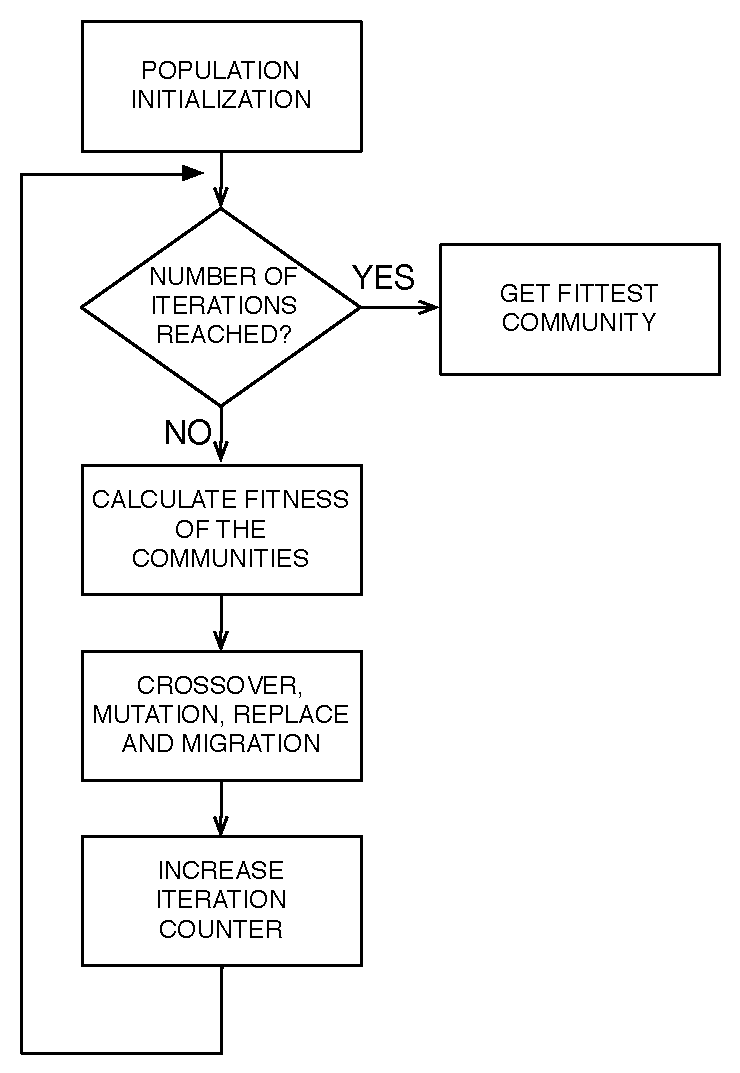
\includegraphics[width=0.70\columnwidth]{figures/flowchart-without/flowchart-without}
\caption{{\label{flowchart-without-dynamic}Flowchart of the Proposed Method with Constant Replace Chance%
}}
\end{center}
\end{figure}

\begin{figure}[h!]
\begin{center}
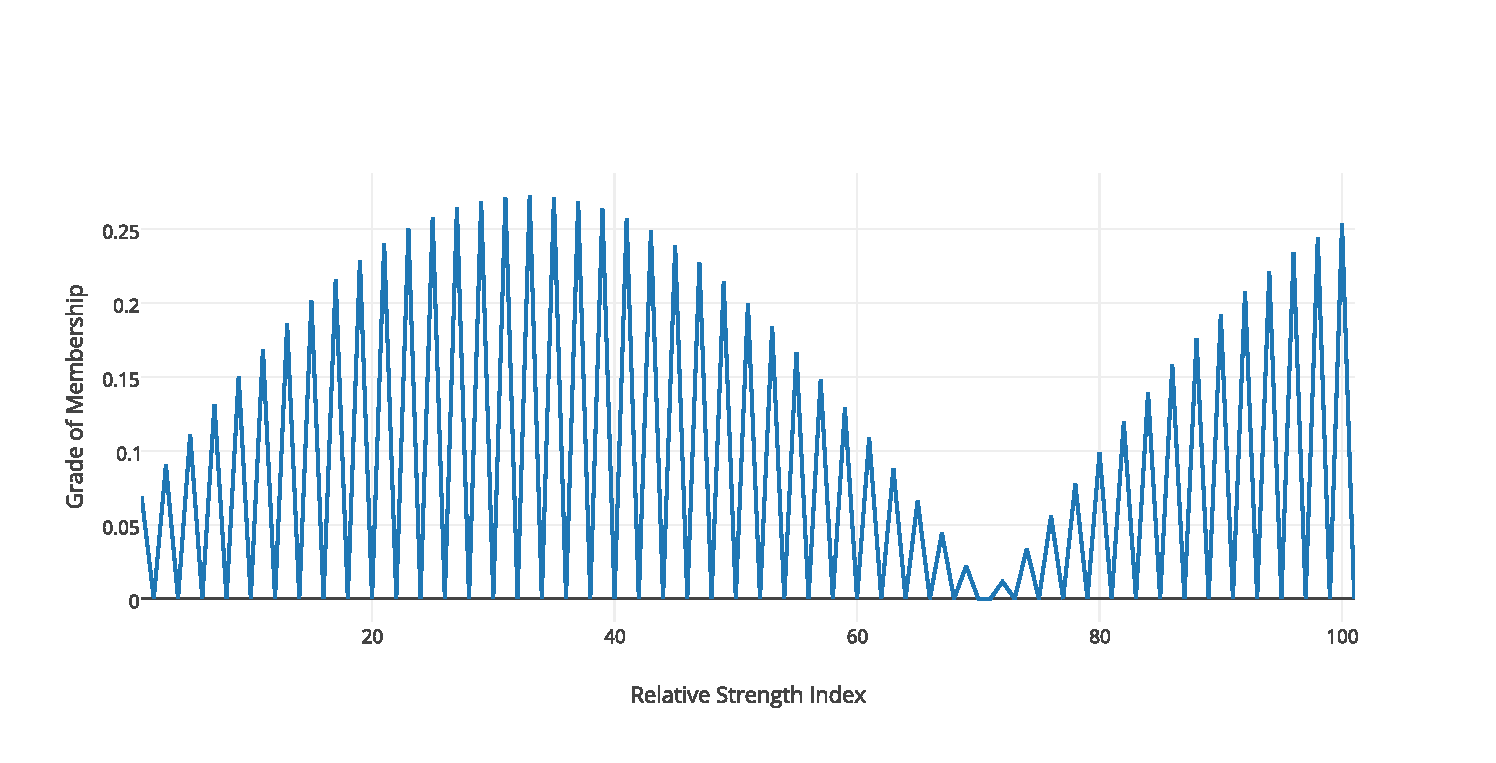
\includegraphics[width=1.00\columnwidth]{figures/mf-input/mf-input}
\caption{{\label{input-mf}Graphical Representation of an Input Membership Function%
}}
\end{center}
\end{figure}

\begin{figure}[h!]
\begin{center}
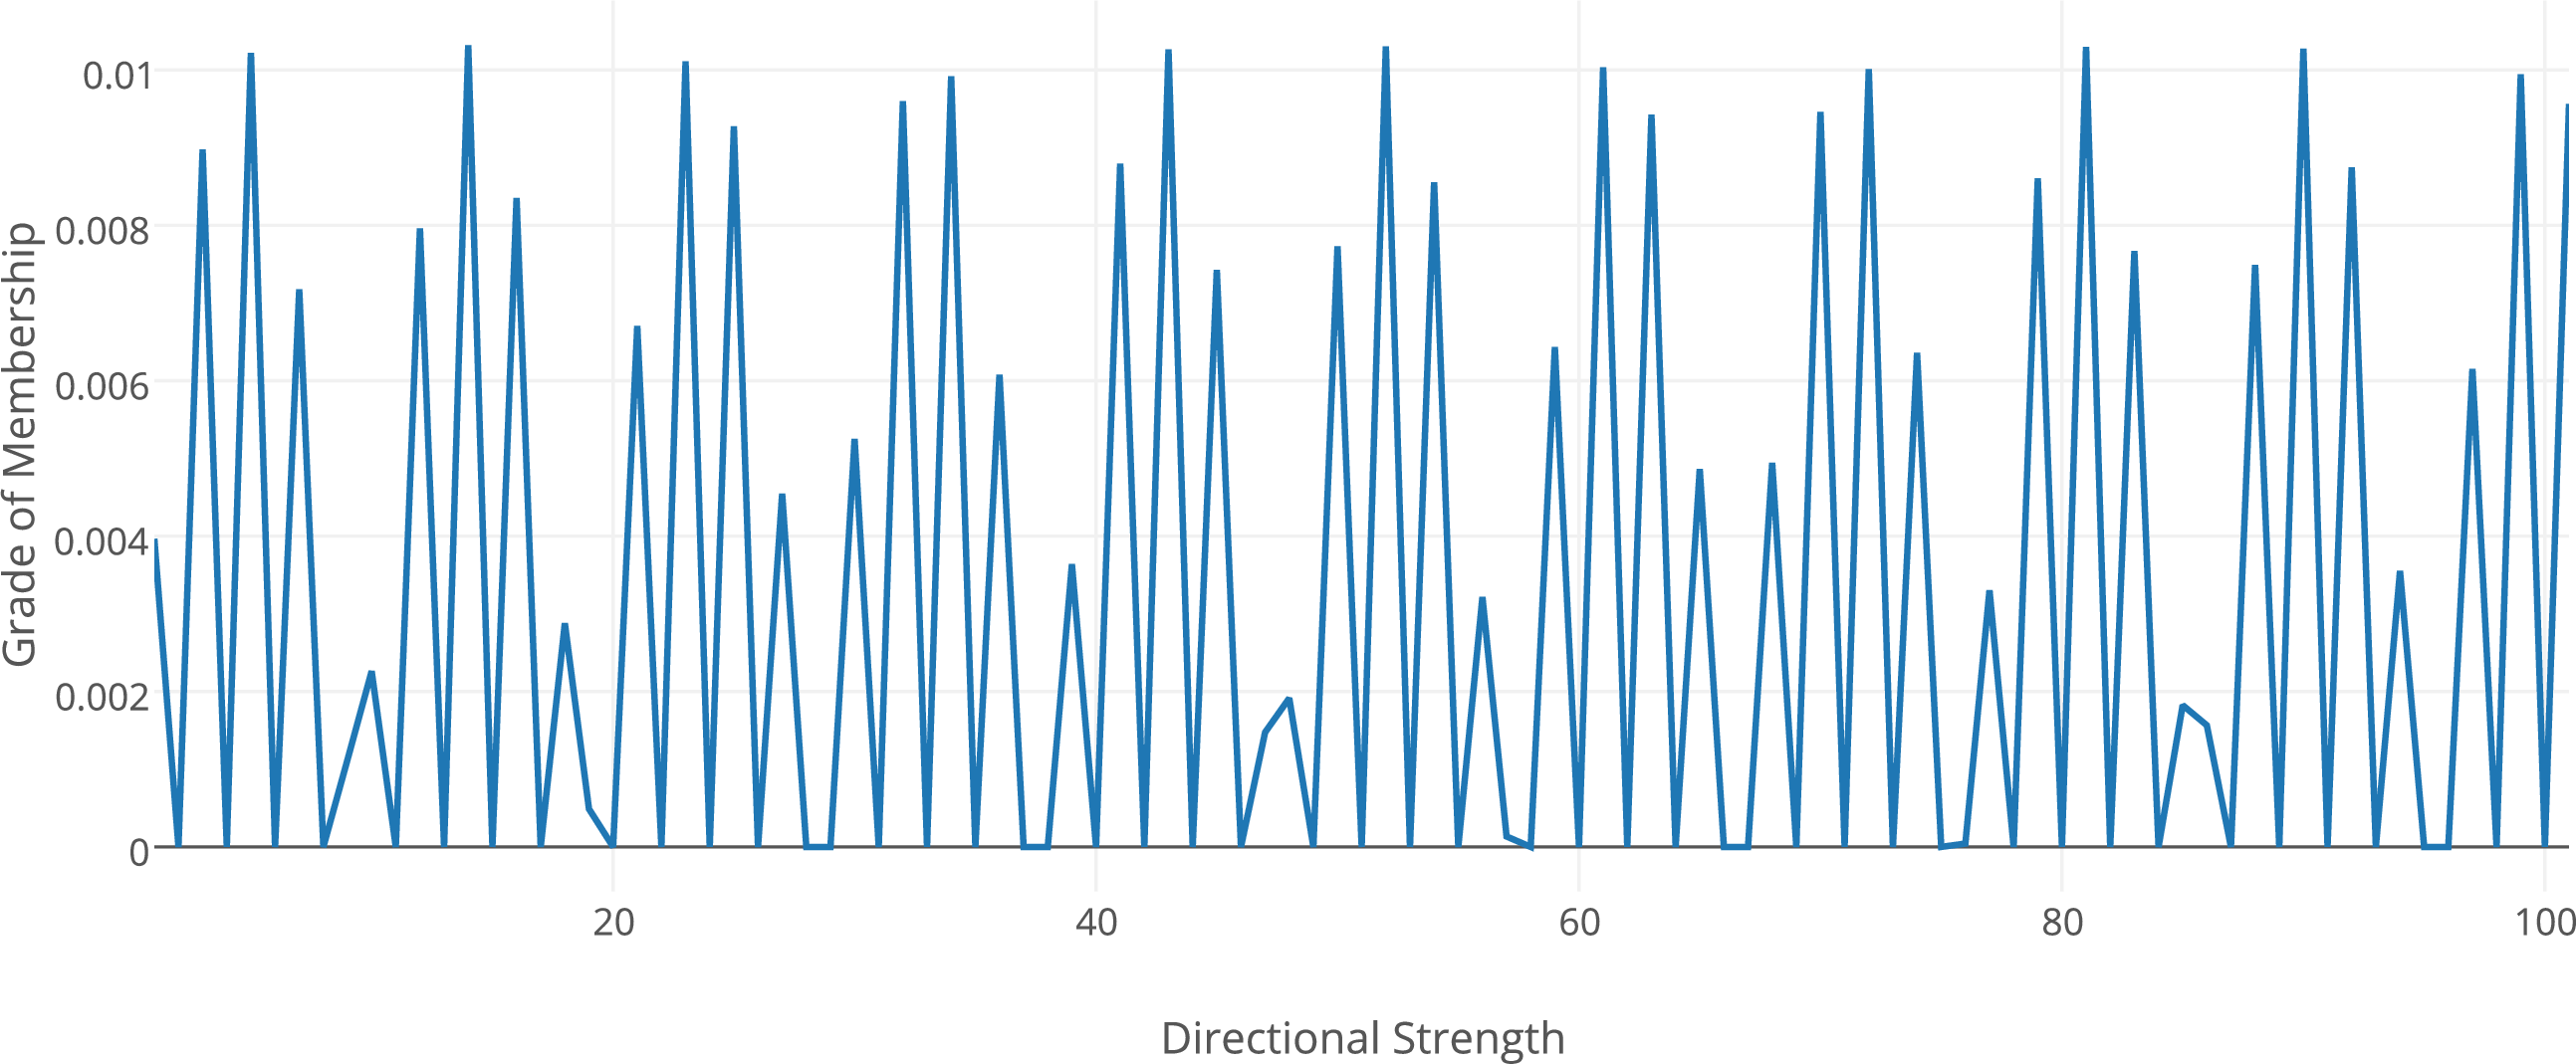
\includegraphics[width=1.00\columnwidth]{figures/mf-output/mf-output}
\caption{{\label{output-mf}Graphical Representation of an Output Membership Function%
}}
\end{center}
\end{figure}

\begin{figure}[h!]
\begin{center}
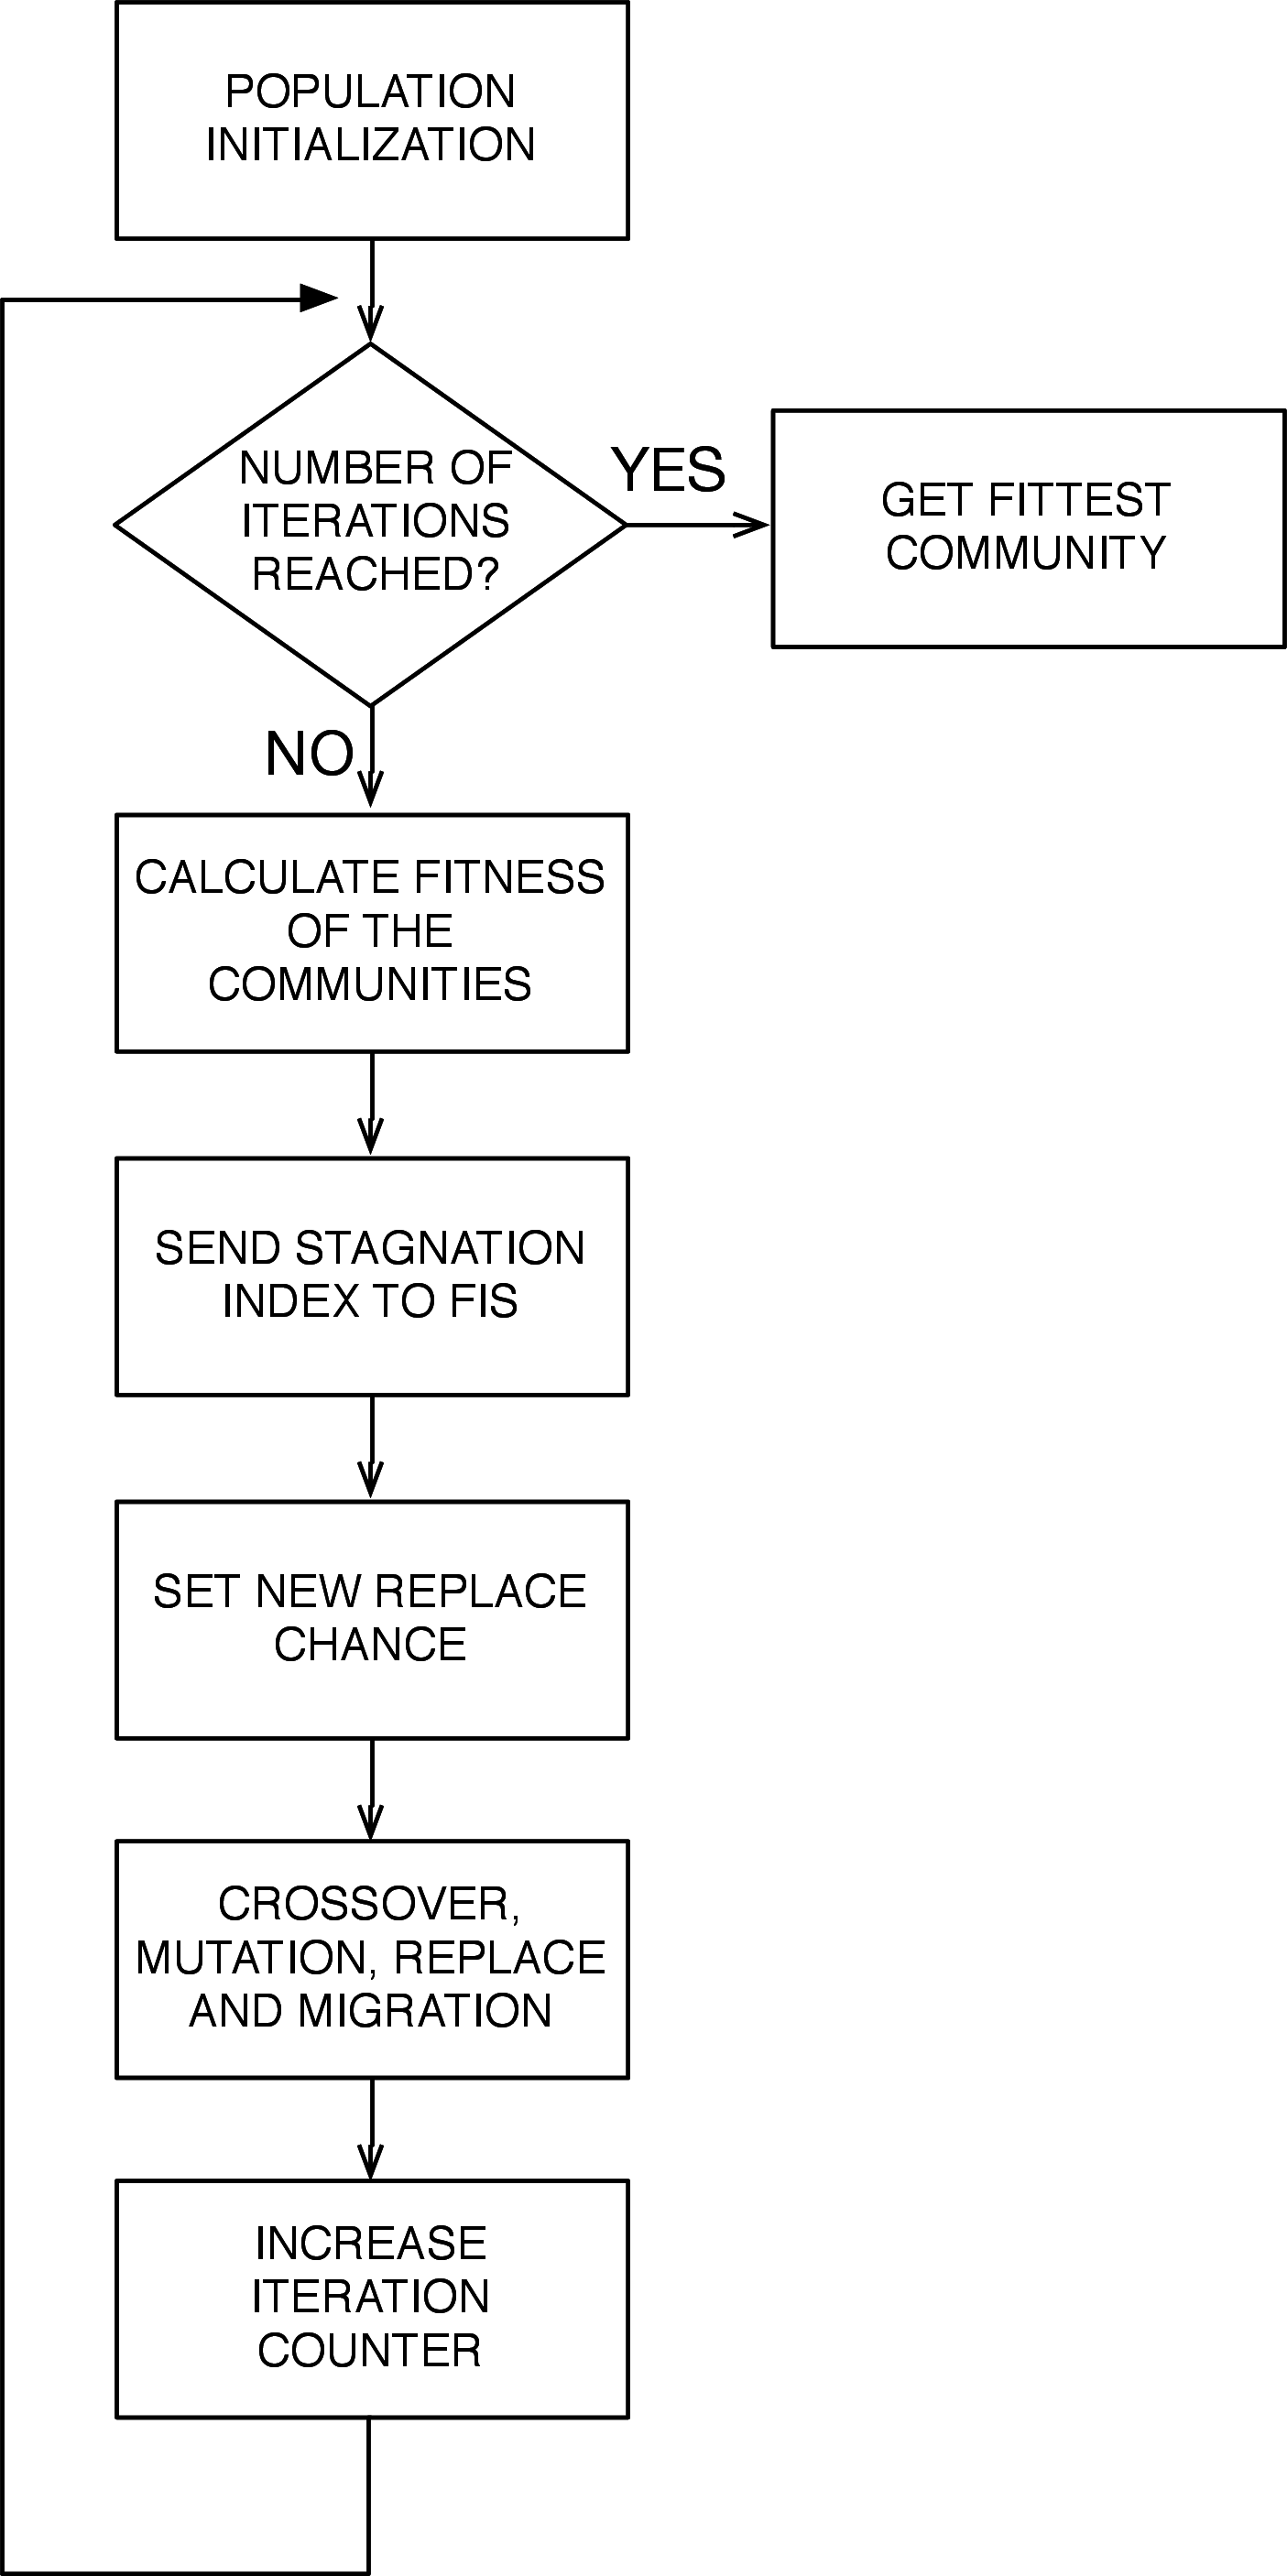
\includegraphics[width=0.70\columnwidth]{figures/flowchart-with/flowchart-with}
\caption{{\label{flowchart-with-dynamic}Flowchart of the Proposed Method with Dynamic Adaptation of Replace Chance%
}}
\end{center}
\end{figure}

\section{Experiments and Results}
\label{experiments-and-results}

This Section begins explaining the experiment and results obtained from implementing the dynamic adaptation of the replace chance through the use of a FIS. Then, the proposed method is compared against the method proposed by Brown, Pelosi, and Dirska \cite{brown2013dynamic}, using their proposed dataset. The experiment by Brown et al., was expanded to 30 trials, instead of 8, in order to obtain more statistical evidence. Furthermore, a series of experiments (where a winning stock has to be chosen, as in the work by Brown, et al.) with an increasing number of generations were performed and, again, 30 trials were run instead of 8, with 30 different number of generations. Another set of experiments similar to the experiments mentioned before were performed, where different configurations of the proposed method are used. Each of the different configurations was run for 30 trials, and the average ROI was collected.

After the previous set of experiments were performed, the authors decided to perform experiments where the forecast of individual stocks take place, instead of choosing a stock to buy for each of the weeks in the dataset. This set of experiments is more a regression type of experiments than a recommendation type. First, five stocks were chosen where the proposed method was applied with different configurations. Then, each of the stocks in the dataset was evaluated with the proposed method using a configuration that was found to have a good performance by trial and error. The effectiveness of the experiments is determined by how much average ROI is collected.

As a final experiment, the proposed method performs a pure regression task, where it tries to predict the directional strength of the next week's record in the dataset.

\subsection{Dynamic Adaptation of the Replace Chance}

To compare the efficacy of the proposed method with, and without dynamic adaptation of the replace chance, two experiments were performed and then compared using a hypothesis test. 30 experiments were run with certain configuration, for 1000 generations each, with a constant value of replace chance. Then, 30 experiments were run with the same configuration, for 1000 generations each, but now with a FIS controlling the replace chance according to the stagnation index explained in Subsection \ref{dynamic-adaptation-of-the-replace-chance}. The error is recorded for each of the 1000 generations, and after one of the experiments is finished, an average of the error for the 1000 generations is calculated. This process is repeated for each of the 60 experiments. Table \ref{dynamic-vs-non-dynamic-table} shows the averages of these experiments.

\begin{table}
    \caption{{Average Errors - Dynamic vs. Fixed Mutation}}
    \label{dynamic-vs-non-dynamic-table}
    \begin{tabular}{ c c | c c}
        \multicolumn{2}{c}{Without Dynamic Adaptation} & \multicolumn{2}{c}{With Dynamic Adaptation} \\ 
         1311.36858  & 1046.104578 & 1216.510814 & 1143.389484 \\ 
         1229.470821 & 1355.991986 & 1241.307708 & 1102.711613 \\ 
         1295.573386 & 1091.08208  & 1120.805705 & 1249.783318 \\ 
         1030.289883 & 1327.723752 & 1172.208267 & 1111.148651 \\ 
         1336.959564 & 1091.20479  & 972.4929395 & 1215.476516 \\ 
         1384.057403 & 1265.682395 & 1170.073256 & 1169.588612 \\ 
         1303.139391 & 1246.964085 & 1278.311636 & 1040.093053 \\ 
         1391.94702  & 1158.730397 & 1154.370559 & 762.2223289 \\ 
         1125.607147 & 1373.704464 & 1063.93828  & 1207.359942 \\ 
         1336.603628 & 1130.282865 & 1227.164144 & 1168.572853 \\
         1308.989252 & 1135.924961 & 1067.38689  & 1162.467748 \\
         1253.008383 & 1384.15463  & 1273.537452 & 1248.3565   \\
         1265.489682 & 1487.437018 & 960.6685944 & 1140.389075 \\
         1247.161813 & 1215.320663 & 1173.268224 & 1309.74542  \\
         1025.353754 & 1173.167377 & 1169.425716 & 978.8573602 \\
    \end{tabular} 
\end{table}

The design of the FIS is rather simple. The input of the FIS is the stagnation index, and the output is the new replace chance for the GP system in that particular iteration or generation. The input MF are depicted in Figure \ref{dynamic-adaptation-input} and the output MF are depicted in Figure \ref{dynamic-adaptation-output}. The design of these MF were obtained according to the subjective opinion of the authors, and by trial and error. The rule set is presented below:

\begin{enumerate}
\item if SI is Low then RC is Low
\item if SI is Medium then RC is Medium
\item if SI is High then RC is High
\end{enumerate}

In Figure \ref{with-vs-without-dynamic}, one can see how the dynamic adaptation of the replace chance helps avoid stagnation of the proposed method. Nevertheless, a hypothesis test was performed to formally prove this hypothesis. The hypothesis test was performed in the statistics software Stata, and the results are shown in Figure \ref{dynamic-hypothesis-test}. One can see that the hypothesis test obtained a t-score of -3.3529, where the critical t value for a 95\% confidence interval is -2.0018. As a conclusion, the null hypothesis is rejected (which is that the average of the error of the 30 averages of the experiments with dynamic adaptation of the replace chance is greater than or equal than the averages without the dynamic adaptation), and this means that the proposed method with dynamic adaptation of the replace chance outperforms the proposed method with a constant value of replace chance.

\subsection{Stock Selection}

In all of the following experiments, the dataset provided in \cite{brown2013dynamic} is used, and the first quarter (12 records) of each stock is used for training, and the second quarter (13 records) is used for testing.

\subsubsection{Comparison Against Brown et al.}

Brown, et al. \cite{brown2013dynamic} used their method to run a set of 8 trials, where the purpose of the experiment is to choose what the algorithm considers will be the better performing stock to buy for the next week. In the end, a single trial sums the rate of return from buying all the stocks that were chosen by the algorithm. In their work, they present a table showing what stocks were chosen and what was the total rate of return of their best trial (which in their case was the 4th trial). Then, they illustrate the results of all the trials in a similar chart to Figure \ref{8-trials}, and they provide an average of the 8 trials.

The authors of this work don't consider this experiment to be enough to prove the efficacy of the proposed method. Nevertheless, we provide an experiment similar to theirs in order to compare results. Table \ref{best-trial-table} shows what stocks our proposed method chose, along with the total rate of return. In this case, it outperformed the results obtained by Brown, et al.
    
\begin{table}
    \caption{{Stocks Selection for Trial 4}} 
    \label{best-trial-table}
    \begin{tabular}{ c c c c c c c }
        Week & Stock & Return &  & Week & Stock & Return \\ 
        1 & MMM & 0.58265 &  & 8 & MMM & 1.27858 \\ 
        2 & HD & 1.92256 &  & 9 & IBM & -2.01259 \\ 
        3 & AA & 3.72861 &  & 10 & INTC & -1.92661 \\ 
        4 & CSCO & 3.48494 &  & 11 & PFE & 0.896414 \\ 
        5 & CSCO & 0.285551 &  & 12 & AA & 3.81731 \\ 
        6 & HD & 0.216626 &  & 13 & PFE & 3.23383 \\ 
        7 & HD & 0.981194 &  & Total &  & 16.489065 \\ 
    \end{tabular}
\end{table}

As mentioned before, Figure \ref{8-trials} shows a graphical representation of the results obtained from the 8 trials, where the quarterly return and the average weekly return are shown. In this case, the average rate of return of the 8 trials was 8.1140\%, which again outperforms the average obtained by Brown, et al., which was 7.075\%.

\subsubsection{Extended Experiments - Constant Configuration, Increasing Generations}

The first extended experiment consists on providing the proposed method certain configuration (4 communities, 4 agents, 3 inputs, and 5 outputs) which was shown to give good results on a trial-and-error manner. This configuration was run 30 times for 30 different values of generations. The results are the average rates of return of the 30 trials, and are depicted in Figure \ref{constant-configuration-generations}. This graph shows that the proposed method tends to get under-trained with a low number of generations, begins to throw good results with a moderate number of generations, and starts to get over-trained with a higher number of generations. With a very high number of generations, the method starts acting chaotically. It is noteworthy to mention that the proposed method never achieved a negative average rate of return.

\subsubsection{Extended Experiments - Variable Configurations}

This experiment is similar to that presented by Brown, et al., with the difference that 30 trials are run instead of 8, and different configurations of the proposed method are used. The results are shown in Table \ref{table-rates-of-return}.

\begin{table}
\caption{{Choosing what Stock to Buy - Variable Configurations}}
\label{table-rates-of-return}
    \begin{tabular}{ c c c c c c }
         & \multicolumn{5}{c}{NUMBER OF AGENTS} \\ 
        GENERATIONS & 1      & 2      & 5      & 10     & 20     \\
            2       & 1.27\% & 2.46\% & 2.33\% & 1.68\% & 2.44\% \\ 
            5       & 3.22\% & 2.57\% & 0.97\% & 2.90\% & 3.70\% \\ 
            10      & 1.82\% & 1.75\% & 3.04\% & 3.19\% & 3.14\% \\ 
            20      & 2.32\% & 1.77\% & 2.28\% & 1.76\% & 4.82\% \\ 
            40      & 3.35\% & 4.07\% & 0.58\% & 4.13\% & 2.53\% \\ 
            80      & 1.48\% & 0.85\% & 3.34\% & 5.61\% & 2.81\% \\ 
    \end{tabular} 
\end{table}

A heatmap is provided in Figure \ref{rates-of-return-heatmap} for the reader in order to better appreciate the results obtained.

\subsubsection{Extended Experiments - Variable Configurations, Predicion of Single Stocks}

In this series of experiments, instead of choosing what stock to buy, a single stock is chosen, and the algorithm had to determine if the trader had to buy or sell that particular stock. The following tables show the rate of return achieved, along with the number of correct predictions (if the trader should sell or buy) enclosed in parentheses. The results are shown for each of the configurations in the following Tables (\ref{aa-ror-table} \ref{csco-ror-table} \ref{ibm-ror-table} \ref{ko-ror-table} \ref{msft-ror-table}), along with corresponding heatmaps (\ref{aa-ror-heatmap} \ref{csco-ror-heatmap} \ref{ibm-ror-heatmap} \ref{ko-ror-heatmap} \ref{msft-ror-heatmap}) that help the reader see what configurations worked better.

\begin{table}
\caption{{American Airlines Rates of Return}}
\label{aa-ror-table}
    \begin{tabular}{ c c c c c }
         & \multicolumn{4}{c}{TRAINING SET SIZE} \\ 
        GENERATIONS & 2           & 4           & 6          & 8           \\ 
        5           & -5.77\% (6) & 6.50\% (8)  & 9.57\% (9) & 12.30\% (8) \\ 
        10          & -5.77\% (6) & 6.50\% (8)  & 7.68\% (8) & 12.30\% (8) \\ 
        15          & -5.77\% (6) & 6.50\% (8)  & 7.68\% (8) & 12.30\% (8) \\ 
        30          & -5.77\% (6) & 14.95\% (9) & 7.68\% (8) & 9.13\% (8)  \\ 
    \end{tabular} 
\end{table}
  
\begin{table}
\caption{{CISCO Rates of Return}}
\label{csco-ror-table}
    \begin{tabular}{ c c c c c }
         & \multicolumn{4}{c}{TRAINING SET SIZE} \\ 
        GENERATIONS & 2           & 4           & 6             & 8           \\ 
        5           & 15.38\% (8) & 26.60\% (10) & 14.42\% (10) & 12.62\% (10) \\ 
        10          & 15.38\% (8) & 26.60\% (10) & 14.42\% (10) & 19.62\% (10) \\ 
        15          & 15.38\% (8) & 26.60\% (10) & 13.46\% (9)  & 15.15\% (9) \\ 
        30          & 13.02\% (7) & 26.60\% (10) & 13.46\% (9)  & 19.62\% (10)  \\ 
    \end{tabular} 
\end{table}

\begin{table}
\caption{{IBM Rates of Return}}
\label{ibm-ror-table}
    \begin{tabular}{ c c c c c }
         & \multicolumn{4}{c}{TRAINING SET SIZE} \\ 
        GENERATIONS & 2            & 4           & 6             & 8           \\ 
        5           & -10.43\% (5) & -12.17\% (5) & 1.65\% (9) & -4.16\% (6) \\ 
        10          & -5.76\% (6)  & -4.18\% (7) & -1.85\% (8) & -2.29\% (6) \\ 
        15          & -9.98\% (6)  & -7.21\% (5) & -6.69\% (7)  & -2.65\% (5) \\ 
        30          & -4.58\% (6)  & -9.61\% (6) & 2.99\% (8)  & -1.10\% (7)  \\ 
    \end{tabular} 
\end{table}

\begin{table}
\caption{{The Coca-Cola Co. Rates of Return}}
\label{ko-ror-table}
    \begin{tabular}{ c c c c c }
         & \multicolumn{4}{c}{TRAINING SET SIZE} \\ 
        GENERATIONS & 2            & 4           & 6             & 8           \\ 
        5           & -8.02\% (5)  & 1.86\% (6)  & 2.19\% (7)    & -1.93\% (7) \\ 
        10          & -9.59\% (4)  & -4.76\% (5) & -3.51\% (7)   & 0.58\% (9) \\ 
        15          & -7.87\% (6)  & -0.81\% (6) & -1.43\% (7)   & 4.69\% (8) \\ 
        30          & -8.02\% (5)  & -8.08\% (5) & -4.43\% (6)   & -7.03\% (6)  \\ 
    \end{tabular} 
\end{table}

\begin{table}
\caption{{Microsoft Rates of Return}}
\label{msft-ror-table}
    \begin{tabular}{ c c c c c }
         & \multicolumn{4}{c}{TRAINING SET SIZE} \\ 
        GENERATIONS & 2            & 4           & 6             & 8           \\ 
        5           & 8.35\% (10)  & 12.26\% (11) & 6.19\% (9)   & -1.52\% (8) \\ 
        10          & 11.82\% (10) & 12.26\% (11) & 1.48\% (7)   & 6.97\% (9) \\ 
        15          & 8.35\% (10)  & 12.26\% (11) & 11.74\% (10) & 6.97\% (9) \\ 
        30          & 8.35\% (10)  & 12.26\% (11) & 11.74\% (10) & 2.42\% (9)  \\ 
    \end{tabular} 
\end{table}

\subsubsection{Extended Experiments - Constant Configuration, Predicion of Every Stock}

Experiments were performed for each of the 30 stocks provided in the dataset. As in previous experiments, 12 weeks were used as training and the next 13 weeks were used for testing. The proposed method tries to predict if the trader has to sell or buy each of the stocks, and for each successful or unsuccessful prediction, a positive or negative rate of return is accumulated, respectively. This process is repeated 30 times for each stock, and the results presented in Table \ref{avg-rates-of-return-table}.

\begin{table}
    \caption{{Average Rate of Return for Each of the 30 Stocks}} 
    \label{avg-rates-of-return-table}
    \begin{tabular}{ c c }
        Stock & Average Rate of Return \\ 
        AA & -0.9178899\% \\ %0
        AXP & -0.09852924\% \\ %1
        BA & 1.2301333\% \\ %2 
        BAC & 9.677296\% \\ %3 
        CAT & -0.029123219\% \\ %4
        CSCO & 1.2233882\% \\ %5
        CVX & -1.7162496\% \\ %6
        DD & 1.6538299\% \\ %7
        DIS & -0.2845998\% \\ %8
        GE & -1.27476446\% \\ %9
        HD & 2.8385108\% \\ %10
        HPQ & -1.2462806\% \\ %11
        IBM & 6.065919\% \\ %12
        INTC & 1.293835\% \\ %13
        JNJ & -2.6360352\% \\ %14
        JPM & -0.8155595\% \\ %15
        KO & 2.2938771\% \\ %16
        KRFT & -0.3530073\% \\ %16
        MCD & -2.8480105\% \\ %17
        MMM & -0.3500379\% \\ %18
        MRK & -6.3991796\% \\ %19
        MSFT & -4.97989\% \\ %20
        PFE & 0.93456393\% \\ %21
        PG & -2.9159548\% \\ %22
        T & 0.061197344\% \\ %23
        TRV & -1.4025264\% \\ %24
        UTX & 1.2724808\% \\ %25
        VZ & -2.7433705\% \\ %26
        WMT & -2.3362381\% \\ %27
        XOM & 1.8770896\% \\ %28
    \end{tabular}
\end{table}
  
\subsubsection{Extended Experiments - Directional Strength Prediction}
  
The final experiment consisted on creating regression models to predict the Directional Strength of a stock. The chosen stock was American Airlines, and the configuration of the Proposed Method was 4 communities, 100 agents per community, 3 inputs (the 3 Technical Indicators), and 5 outputs. The high number of agents was chosen to demonstrate how the method behaves with such a higher number. Three experiments were performed: the first one was run for 10 generations, the second one for 100 generations, and the third one for 1000 generations. The objective of this experiment was to demonstrate that with higher generations, the method can decrease the error. The objective was achieved, as can be seen in Table \ref{ds-mse-table}. The curve-fitting charts can be found in Figure \ref{ds-prediction-10} (10 generations), Figure \ref{ds-prediction-100} (100 generations), and Figure \ref{ds-prediction-1000} (1000 generations).

\begin{table}
    \caption{{Directional Strength Prediction}}
    \label{ds-mse-table}
    \begin{tabular}{ c c }
        Generations & abs(MSE + sum of forces) \\ 
        10 & 4430.62 \\ 
        100 & 2573.73 \\ 
        1000 & 2310.74 \\ 
    \end{tabular} 
\end{table}
  
  
  
  
  
  
  
  
  
  
  
  
  
  
  
  
  
  
  
  
  
  
  
  
  
  
  
  
  
  
  
  
  
  
  
  
  
  
  
  
  
  
  
  
  

\begin{figure}[h!]
\begin{center}
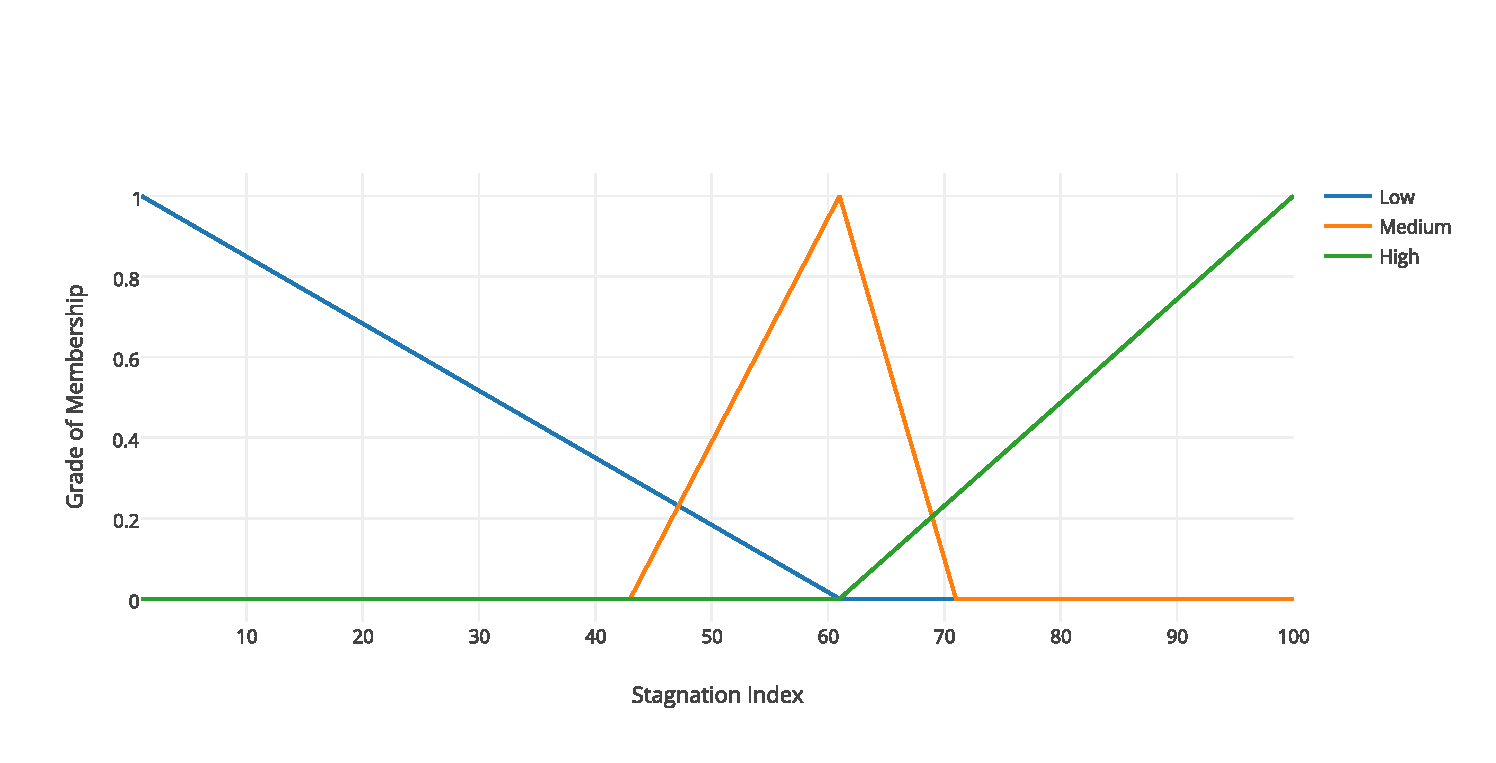
\includegraphics[width=1.00\columnwidth]{figures/stagnation-input/stagnation-input}
\caption{{\label{dynamic-adaptation-input}Input for the Dynamic Adaptation of the Replace Chance%
}}
\end{center}
\end{figure}

\begin{figure}[h!]
\begin{center}
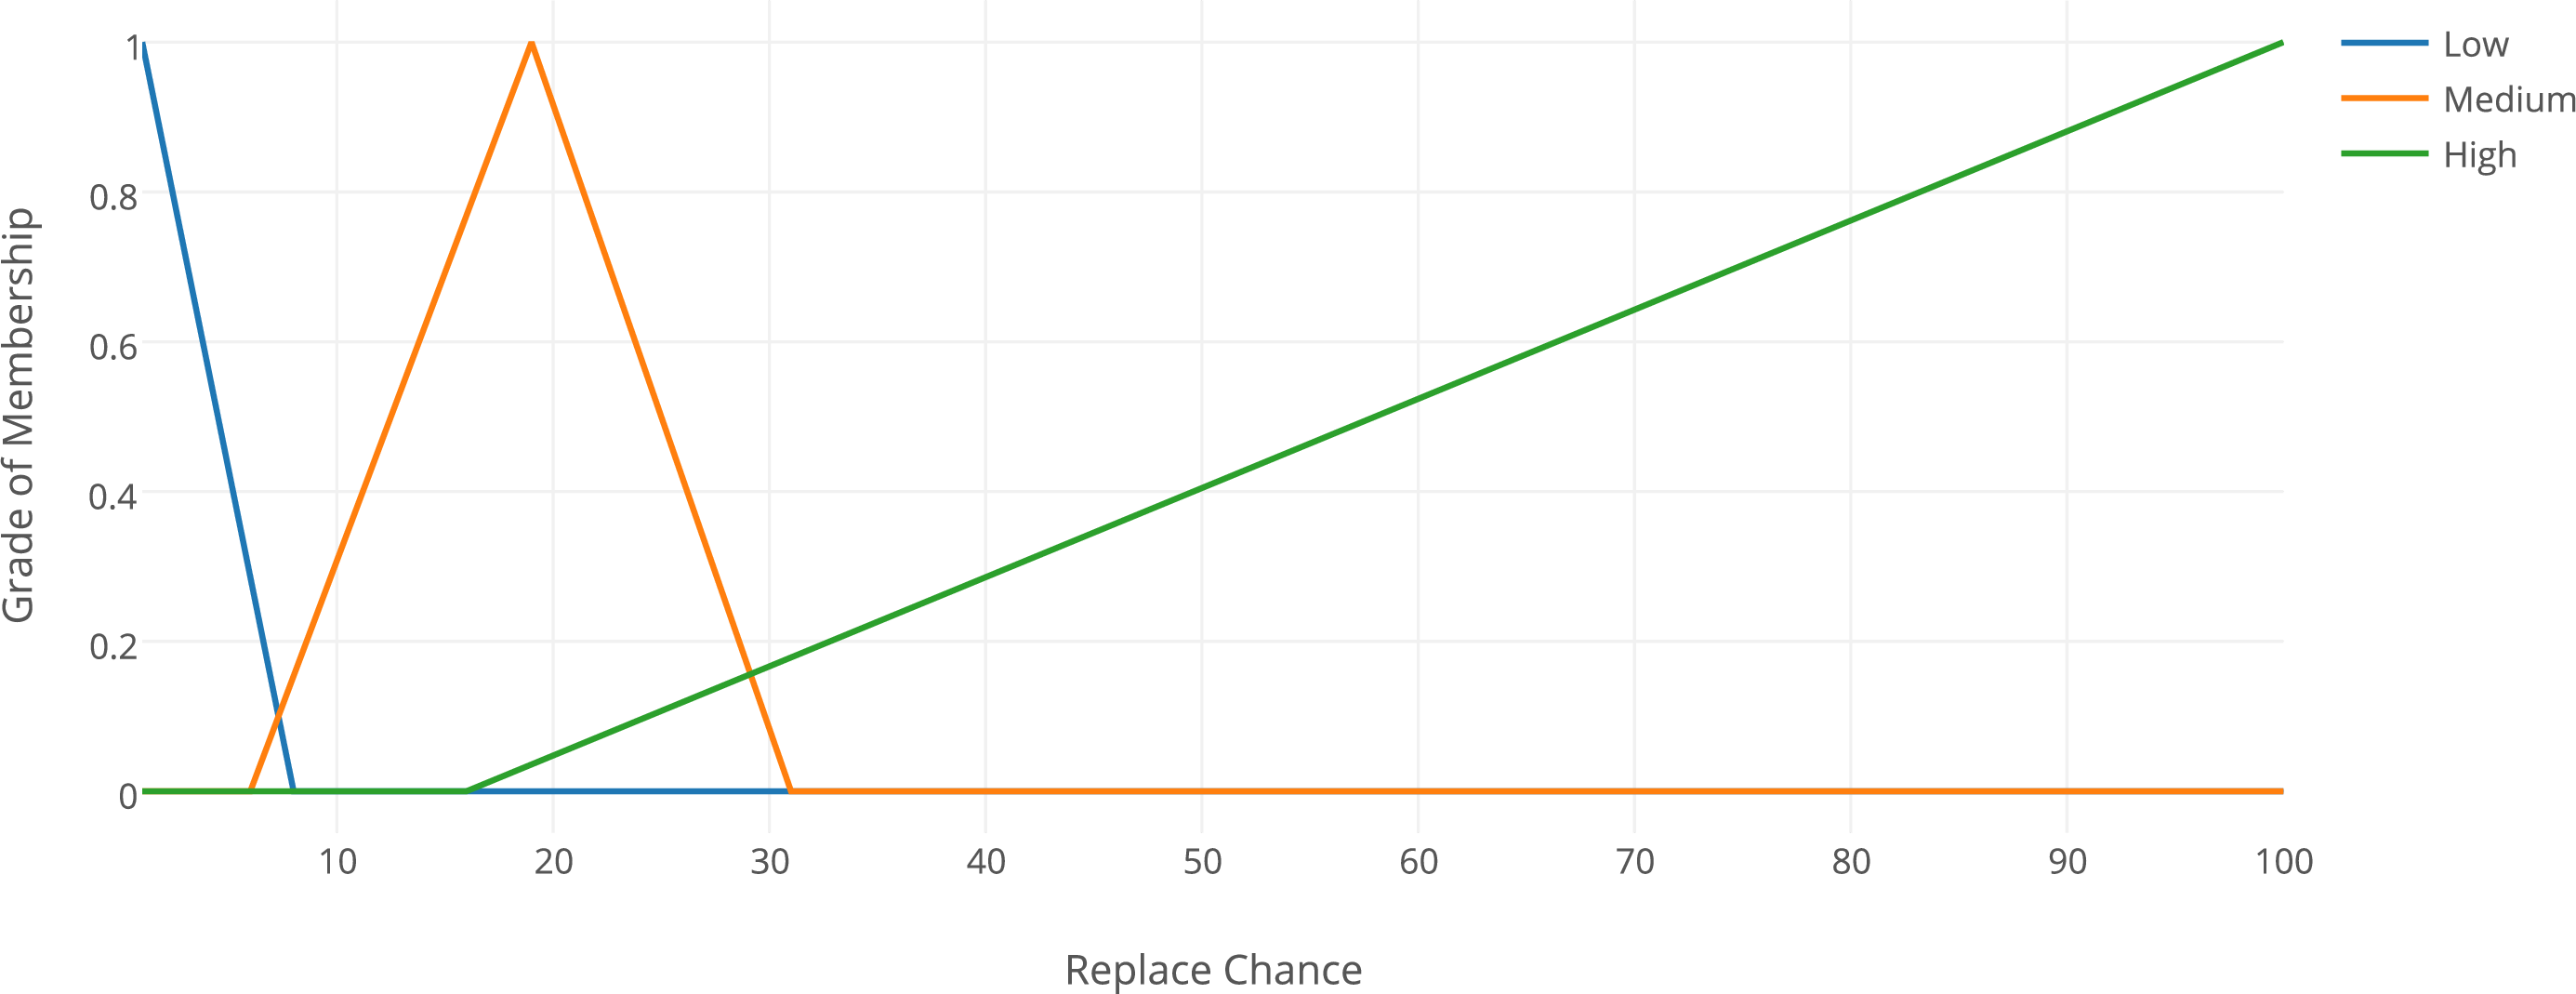
\includegraphics[width=1.00\columnwidth]{figures/stagnation-output/stagnation-output}
\caption{{\label{dynamic-adaptation-output}Output for the Dynamic Adaptation of the Replace Chance%
}}
\end{center}
\end{figure}

\begin{figure}[h!]
\begin{center}
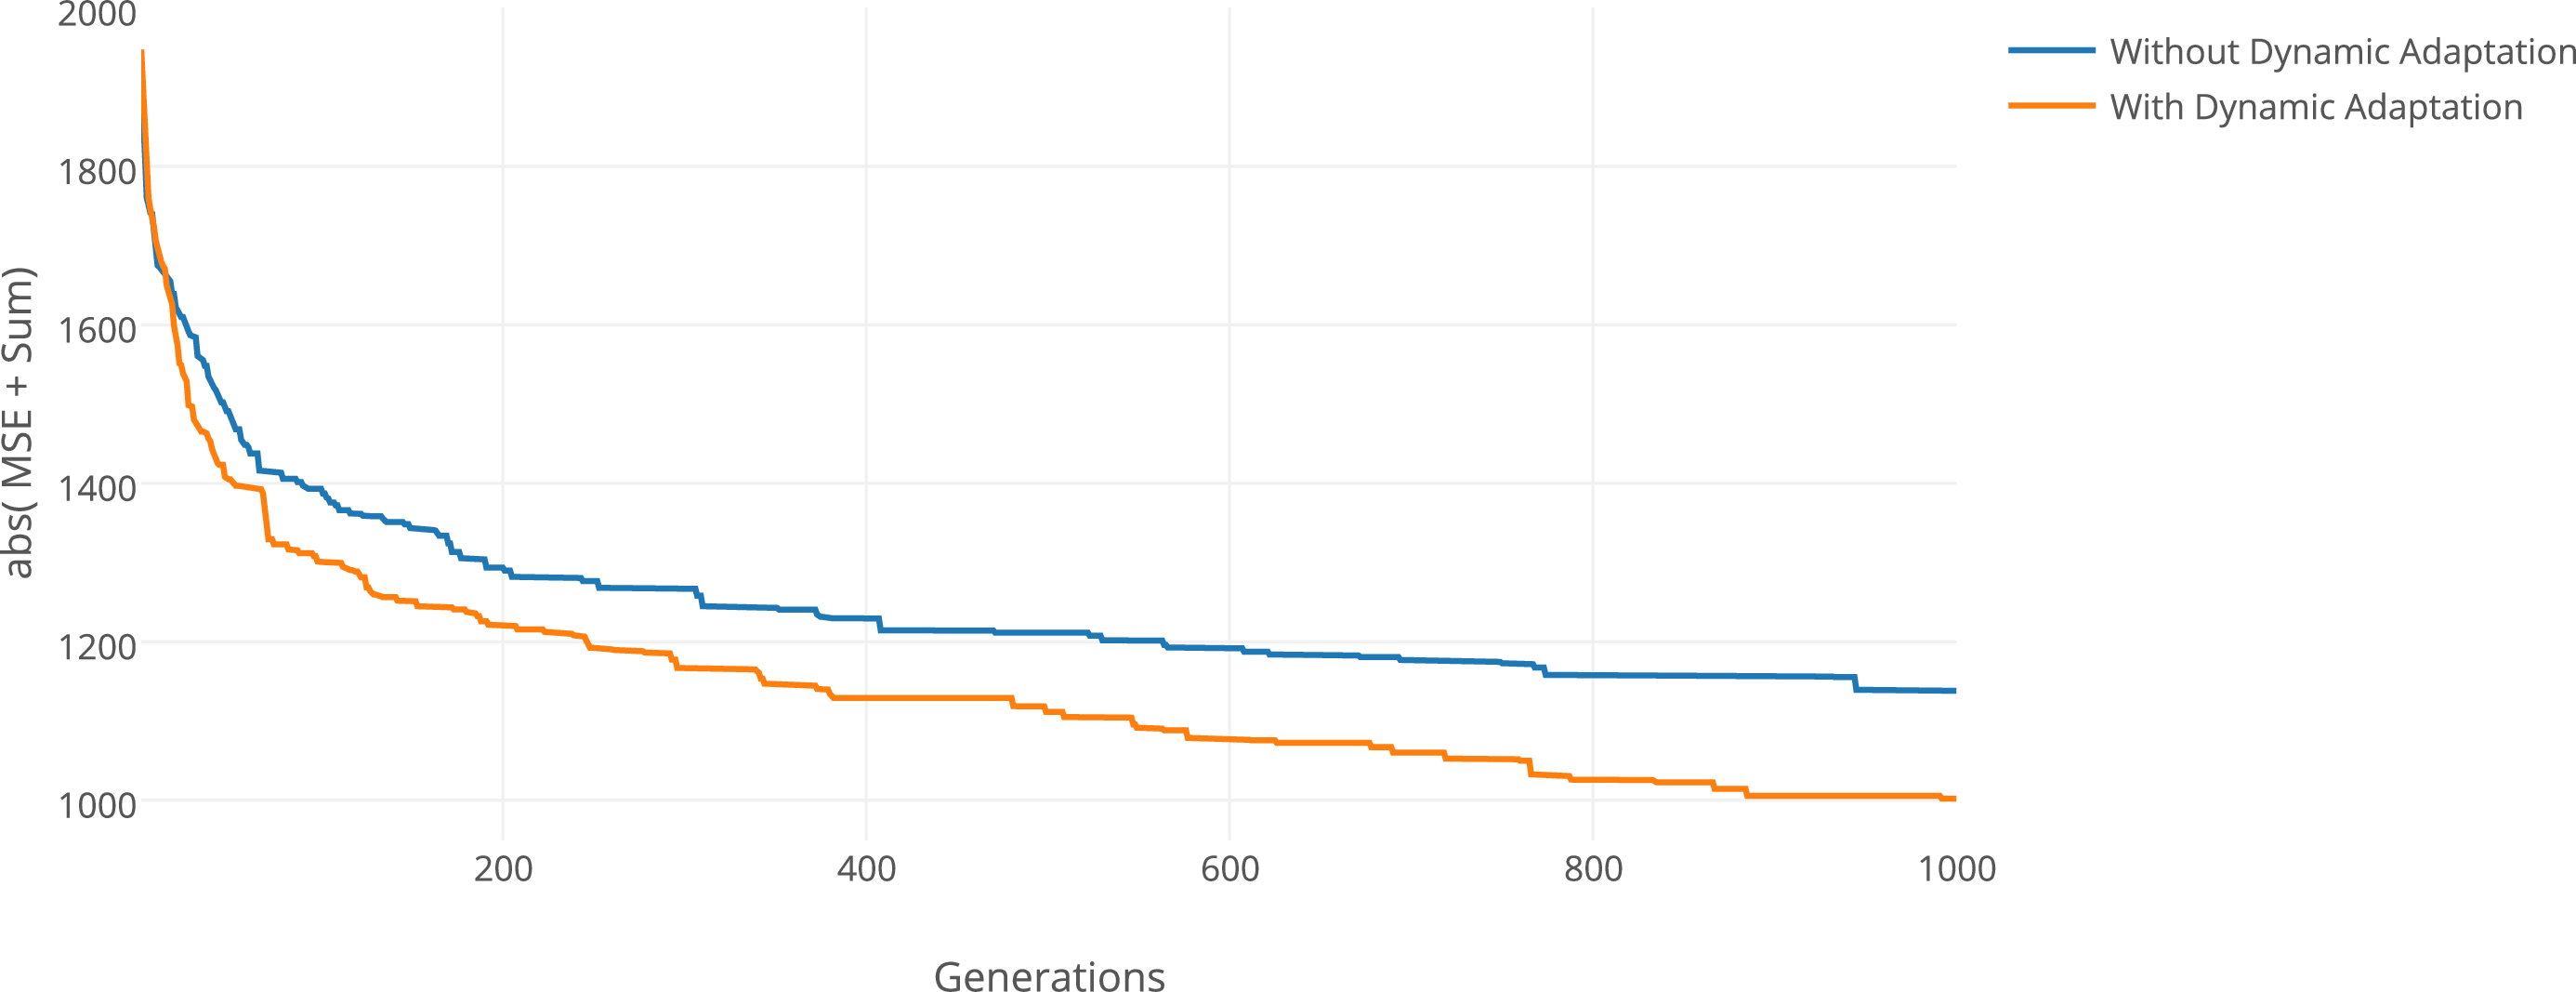
\includegraphics[width=1.00\columnwidth]{figures/fis-vs-no-fis/fis-vs-no-fis}
\caption{{\label{with-vs-without-dynamic}Dynamic Adaptation of Replace Chance vs Constant Replace Chance%
}}
\end{center}
\end{figure}

\begin{figure}[h!]
\begin{center}
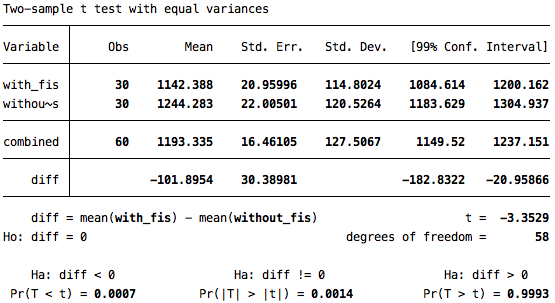
\includegraphics[width=1.00\columnwidth]{figures/dynamic-parameter-statistical-test/dynamic-parameter-statistical-test}
\caption{{\label{dynamic-hypothesis-test}Hypothesis Test for the Dynamic Adaptation of the Replace Chance%
}}
\end{center}
\end{figure}

\begin{figure}[h!]
\begin{center}
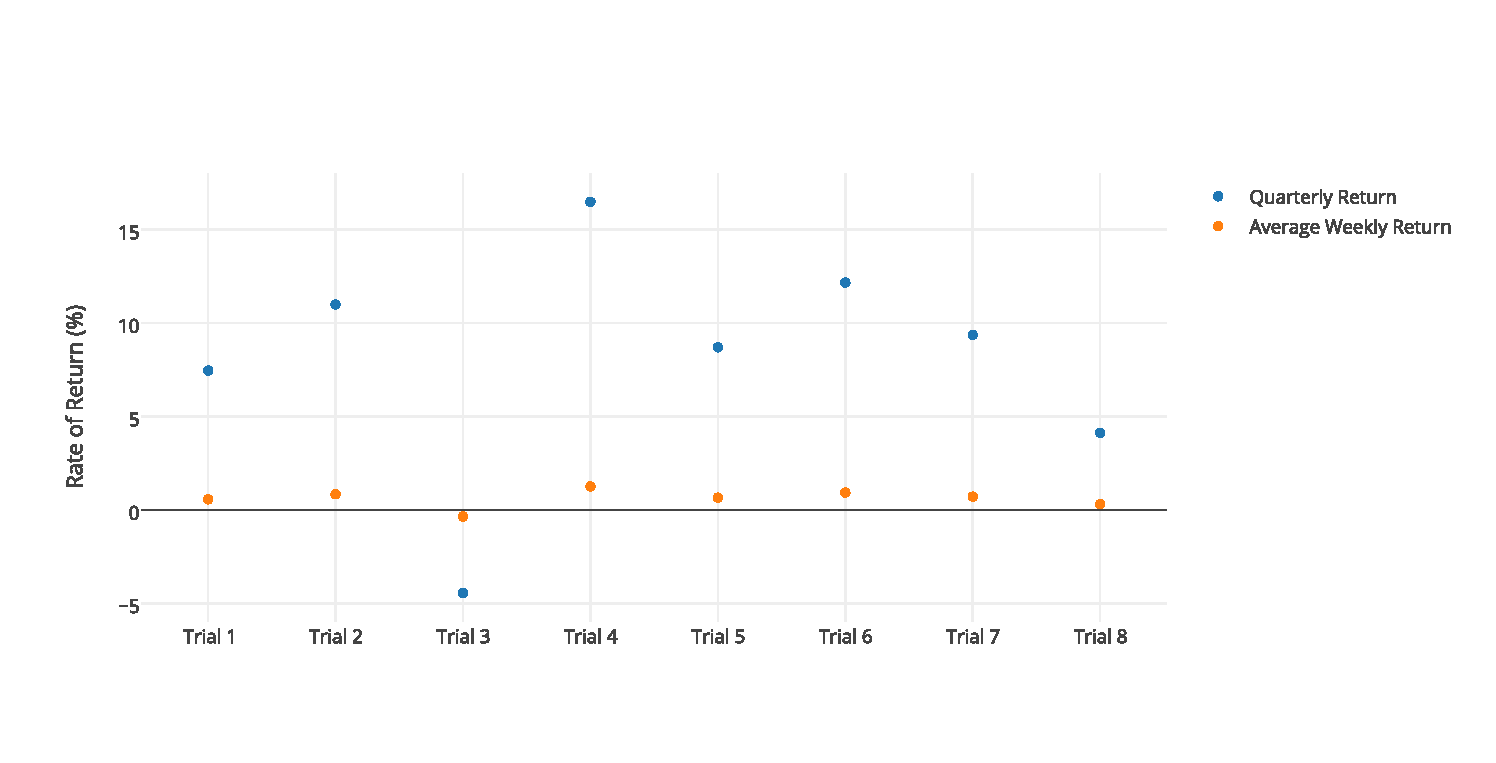
\includegraphics[width=1.00\columnwidth]{figures/percent-return-per-trial/percent-return-per-trial}
\caption{{\label{8-trials}Rate of Return of the 8 Trials%
}}
\end{center}
\end{figure}

\begin{figure}[h!]
\begin{center}
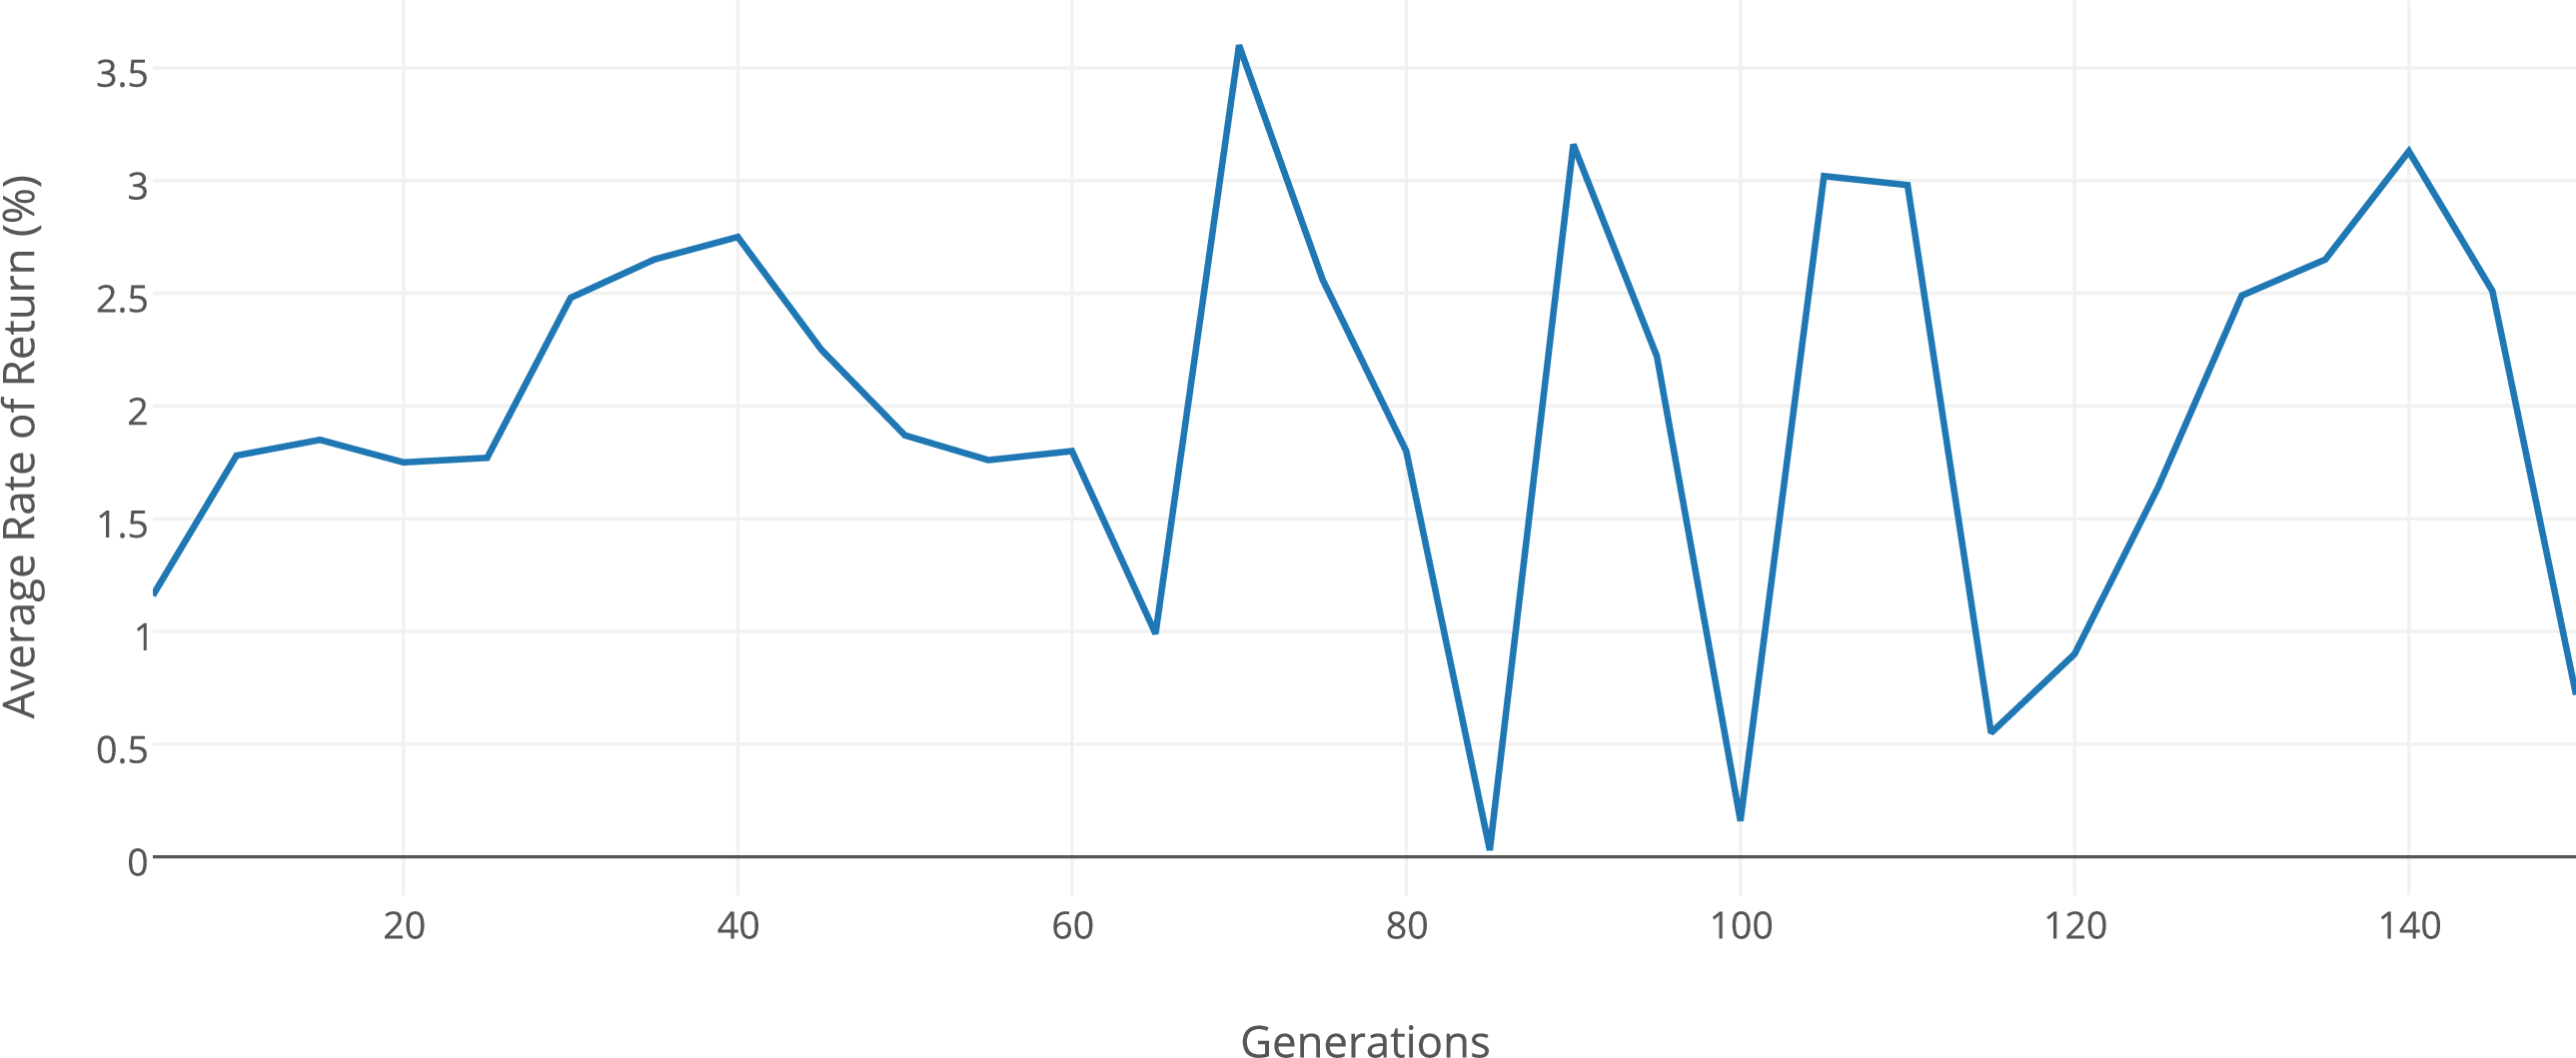
\includegraphics[width=1.00\columnwidth]{figures/avg-rate-of-return/avg-rate-of-return}
\caption{{\label{constant-configuration-generations}Experiments of the Proposed Method with a Constant Configuration and Increasing Generations%
}}
\end{center}
\end{figure}

\begin{figure}[h!]
\begin{center}
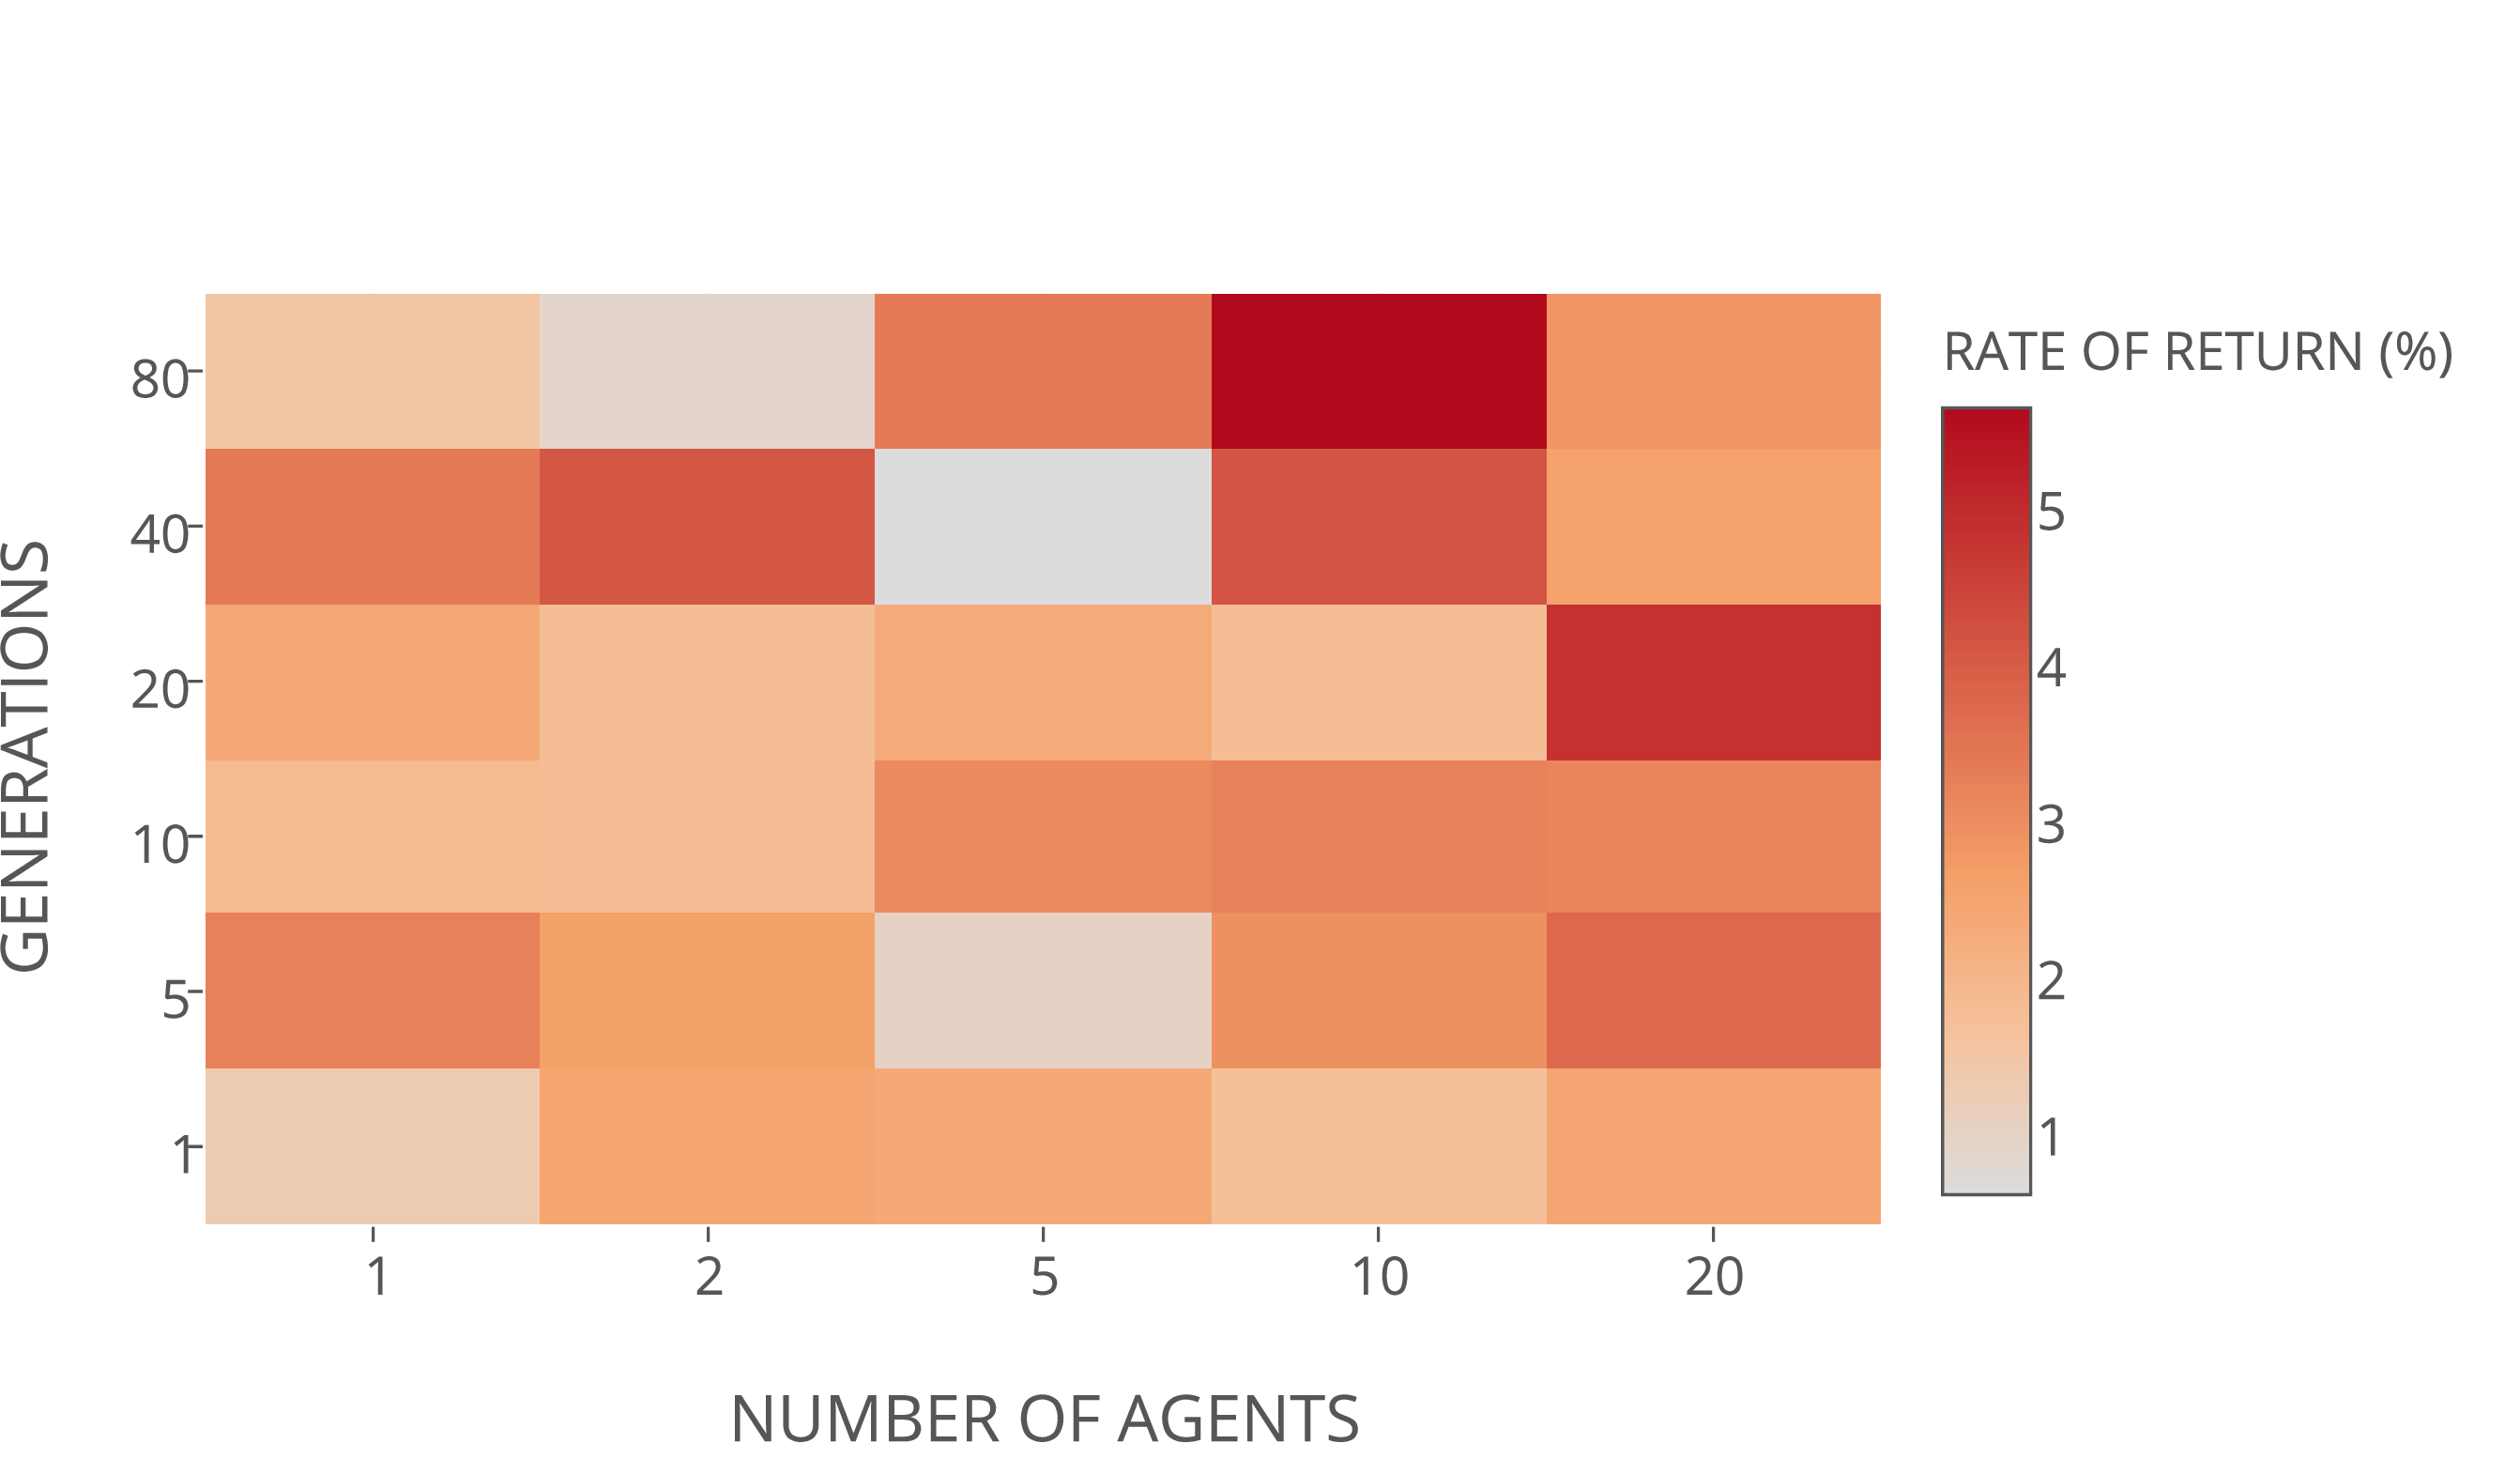
\includegraphics[width=1.00\columnwidth]{figures/rates-of-return-heatmap/rates-of-return-heatmap}
\caption{{\label{rates-of-return-heatmap}What stock to choose%
}}
\end{center}
\end{figure}

\begin{figure}[h!]
\begin{center}
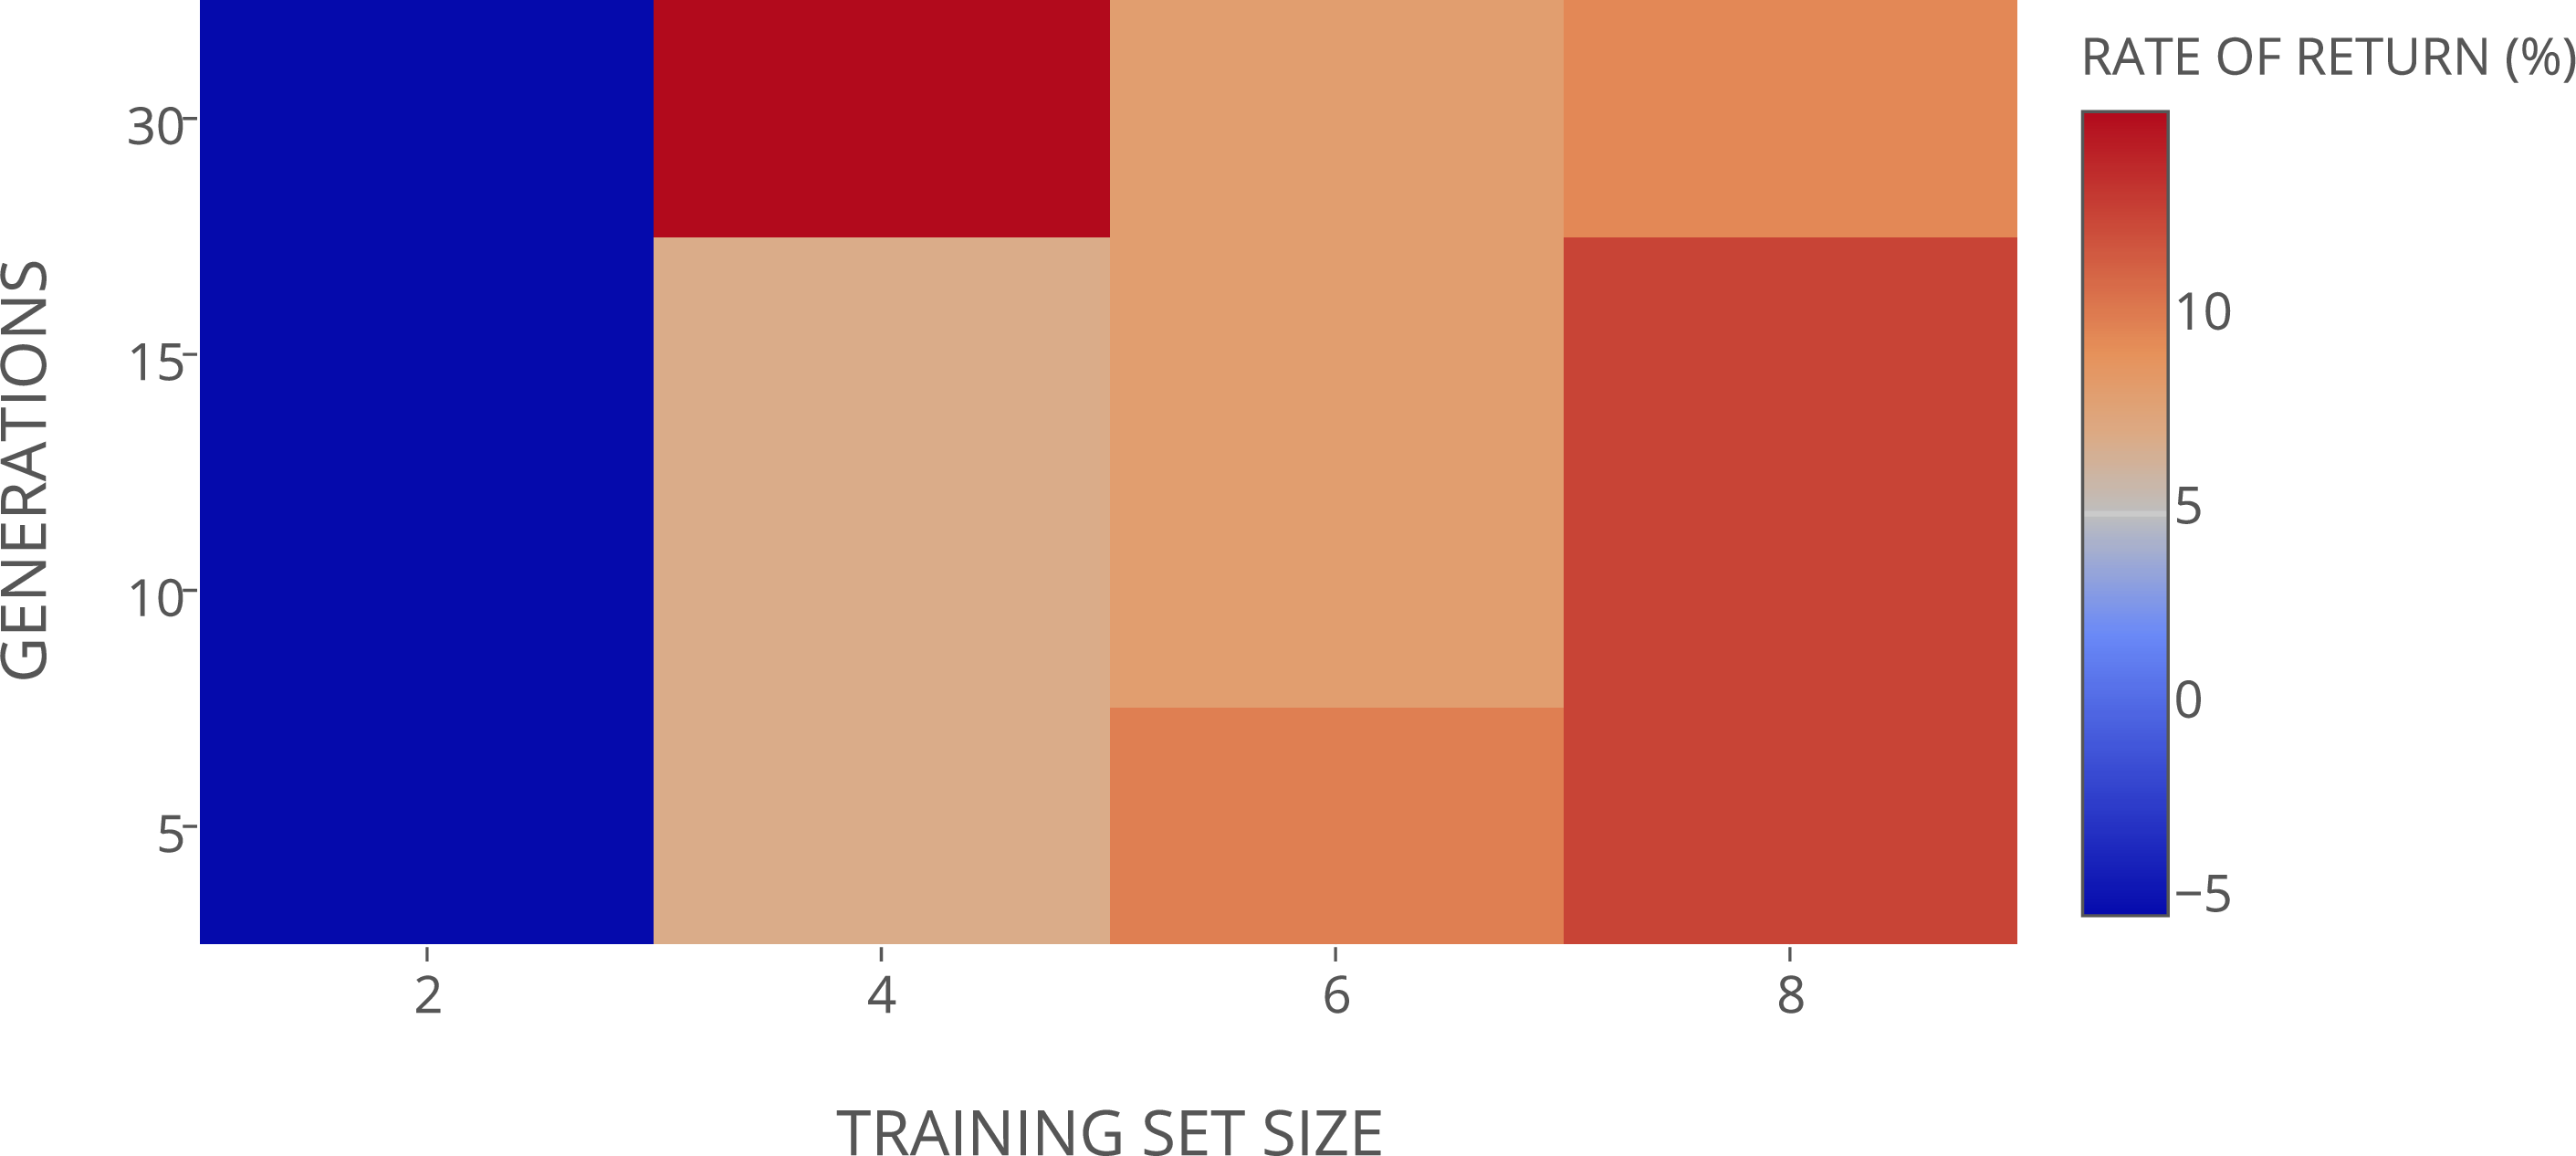
\includegraphics[width=1.00\columnwidth]{figures/rates-of-return-aa-heatmap/rates-of-return-aa-heatmap}
\caption{{\label{aa-ror-heatmap}American Airlines Rates of Return Heatmap%
}}
\end{center}
\end{figure}

\begin{figure}[h!]
\begin{center}
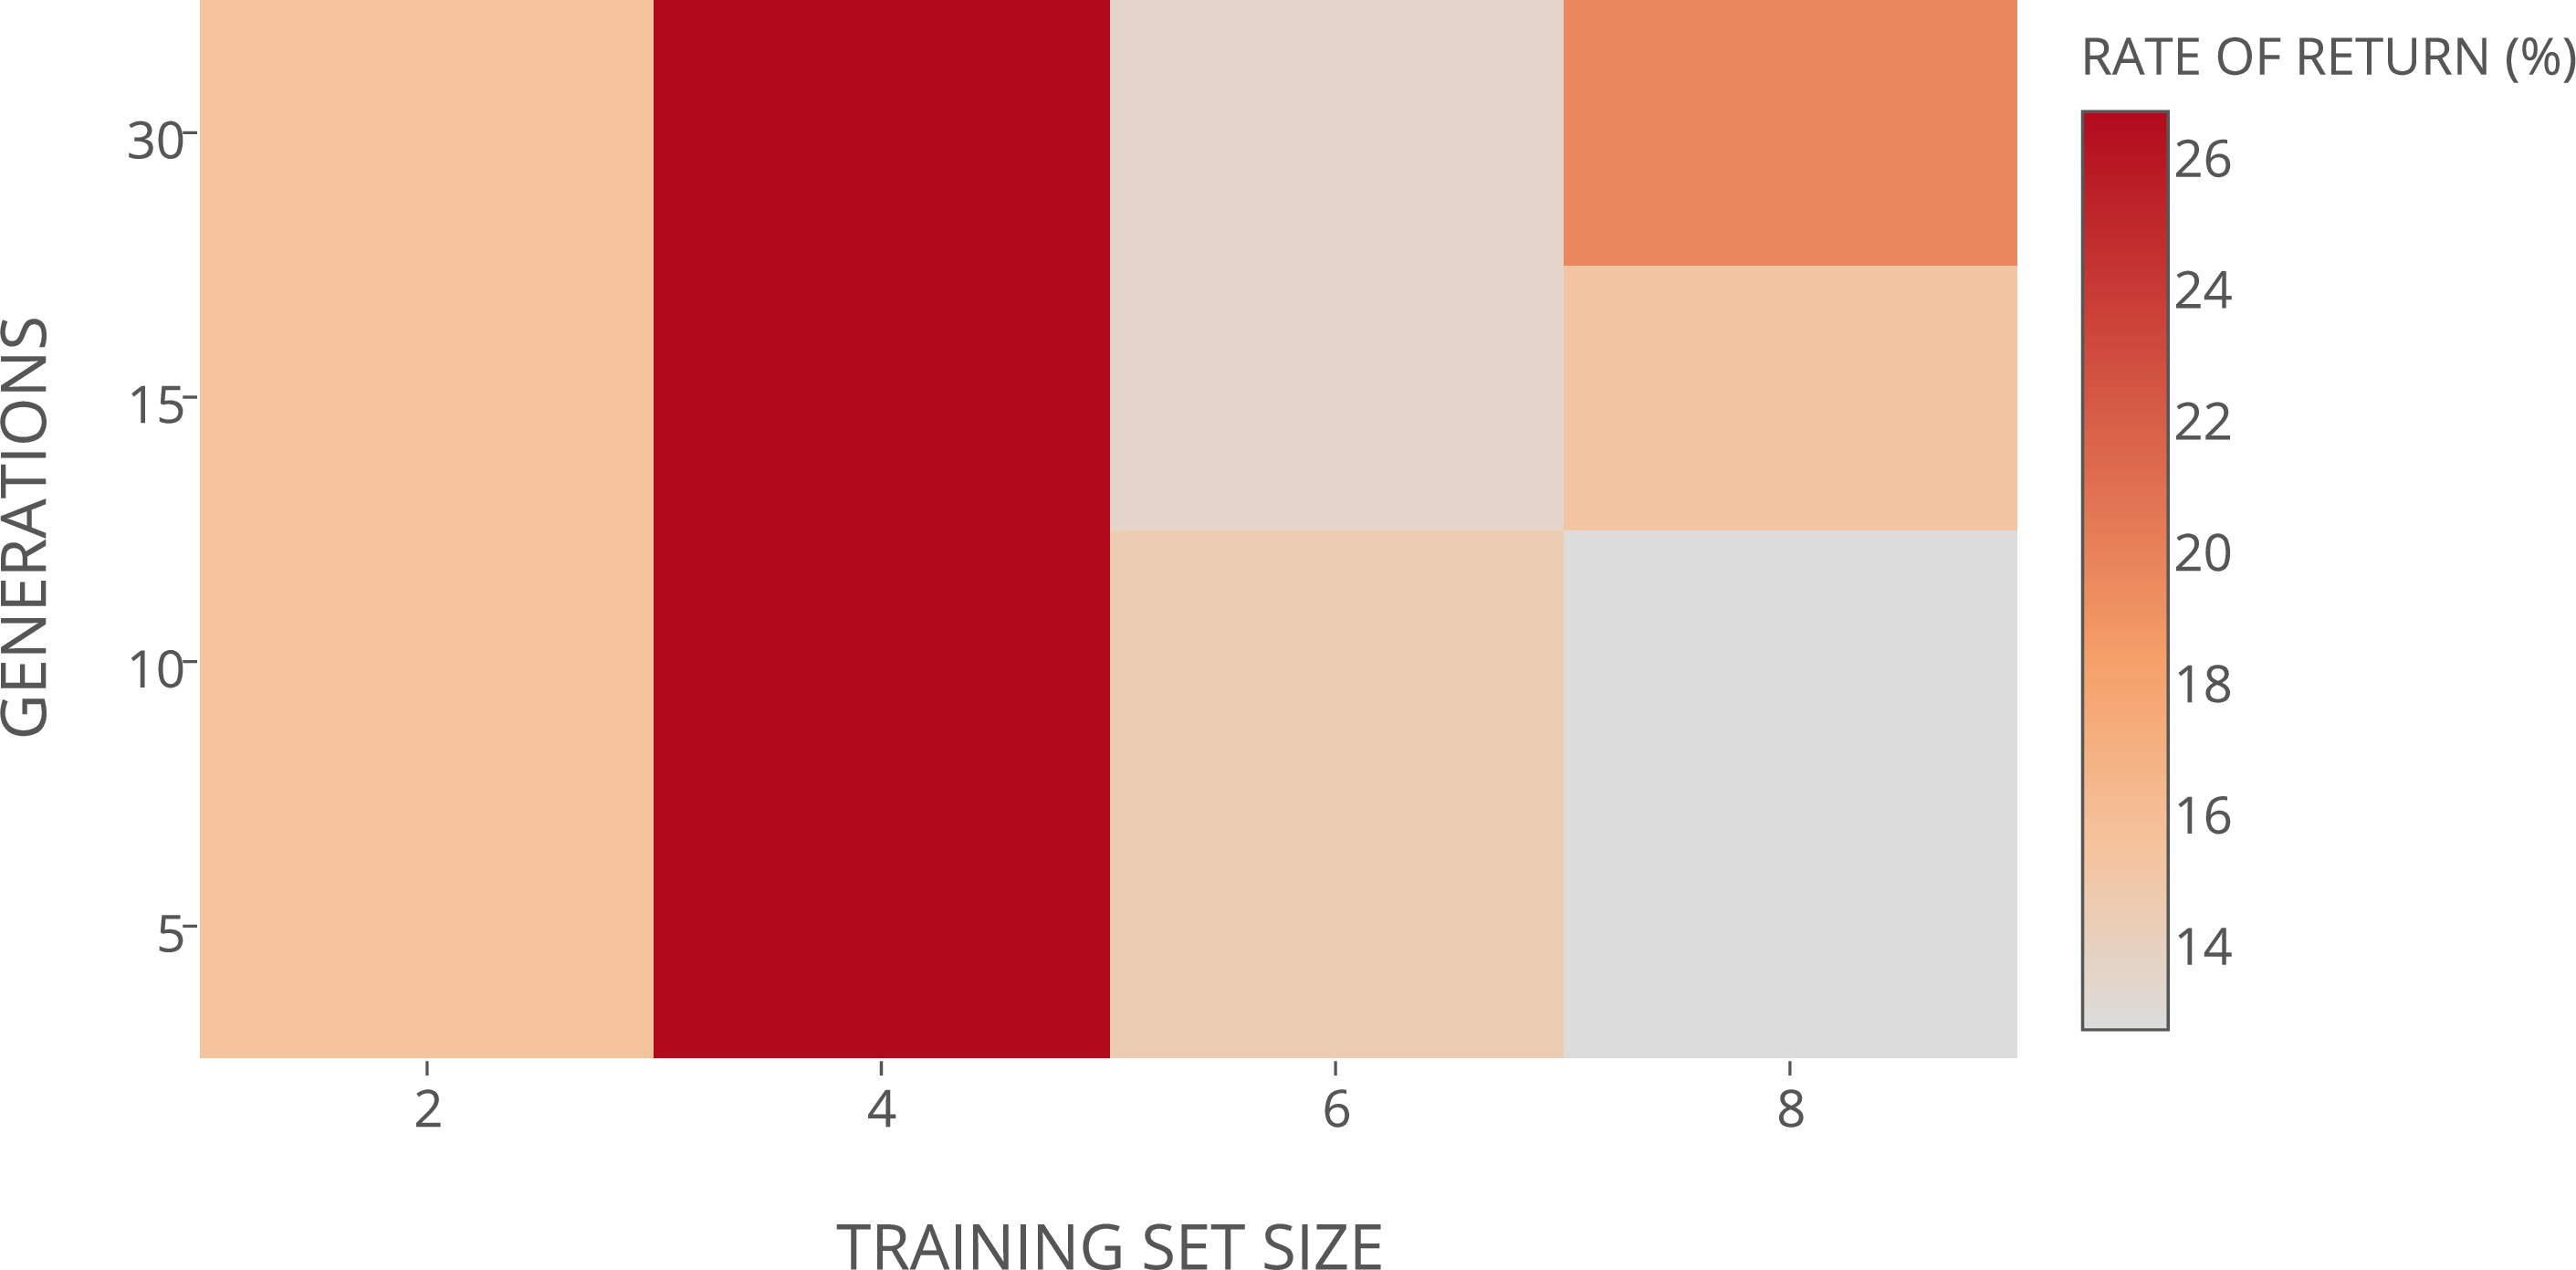
\includegraphics[width=1.00\columnwidth]{figures/rates-of-return-csco-heatmap/rates-of-return-csco-heatmap}
\caption{{\label{csco-ror-heatmap}CISCO Rates of Return Heatmap%
}}
\end{center}
\end{figure}

\begin{figure}[h!]
\begin{center}
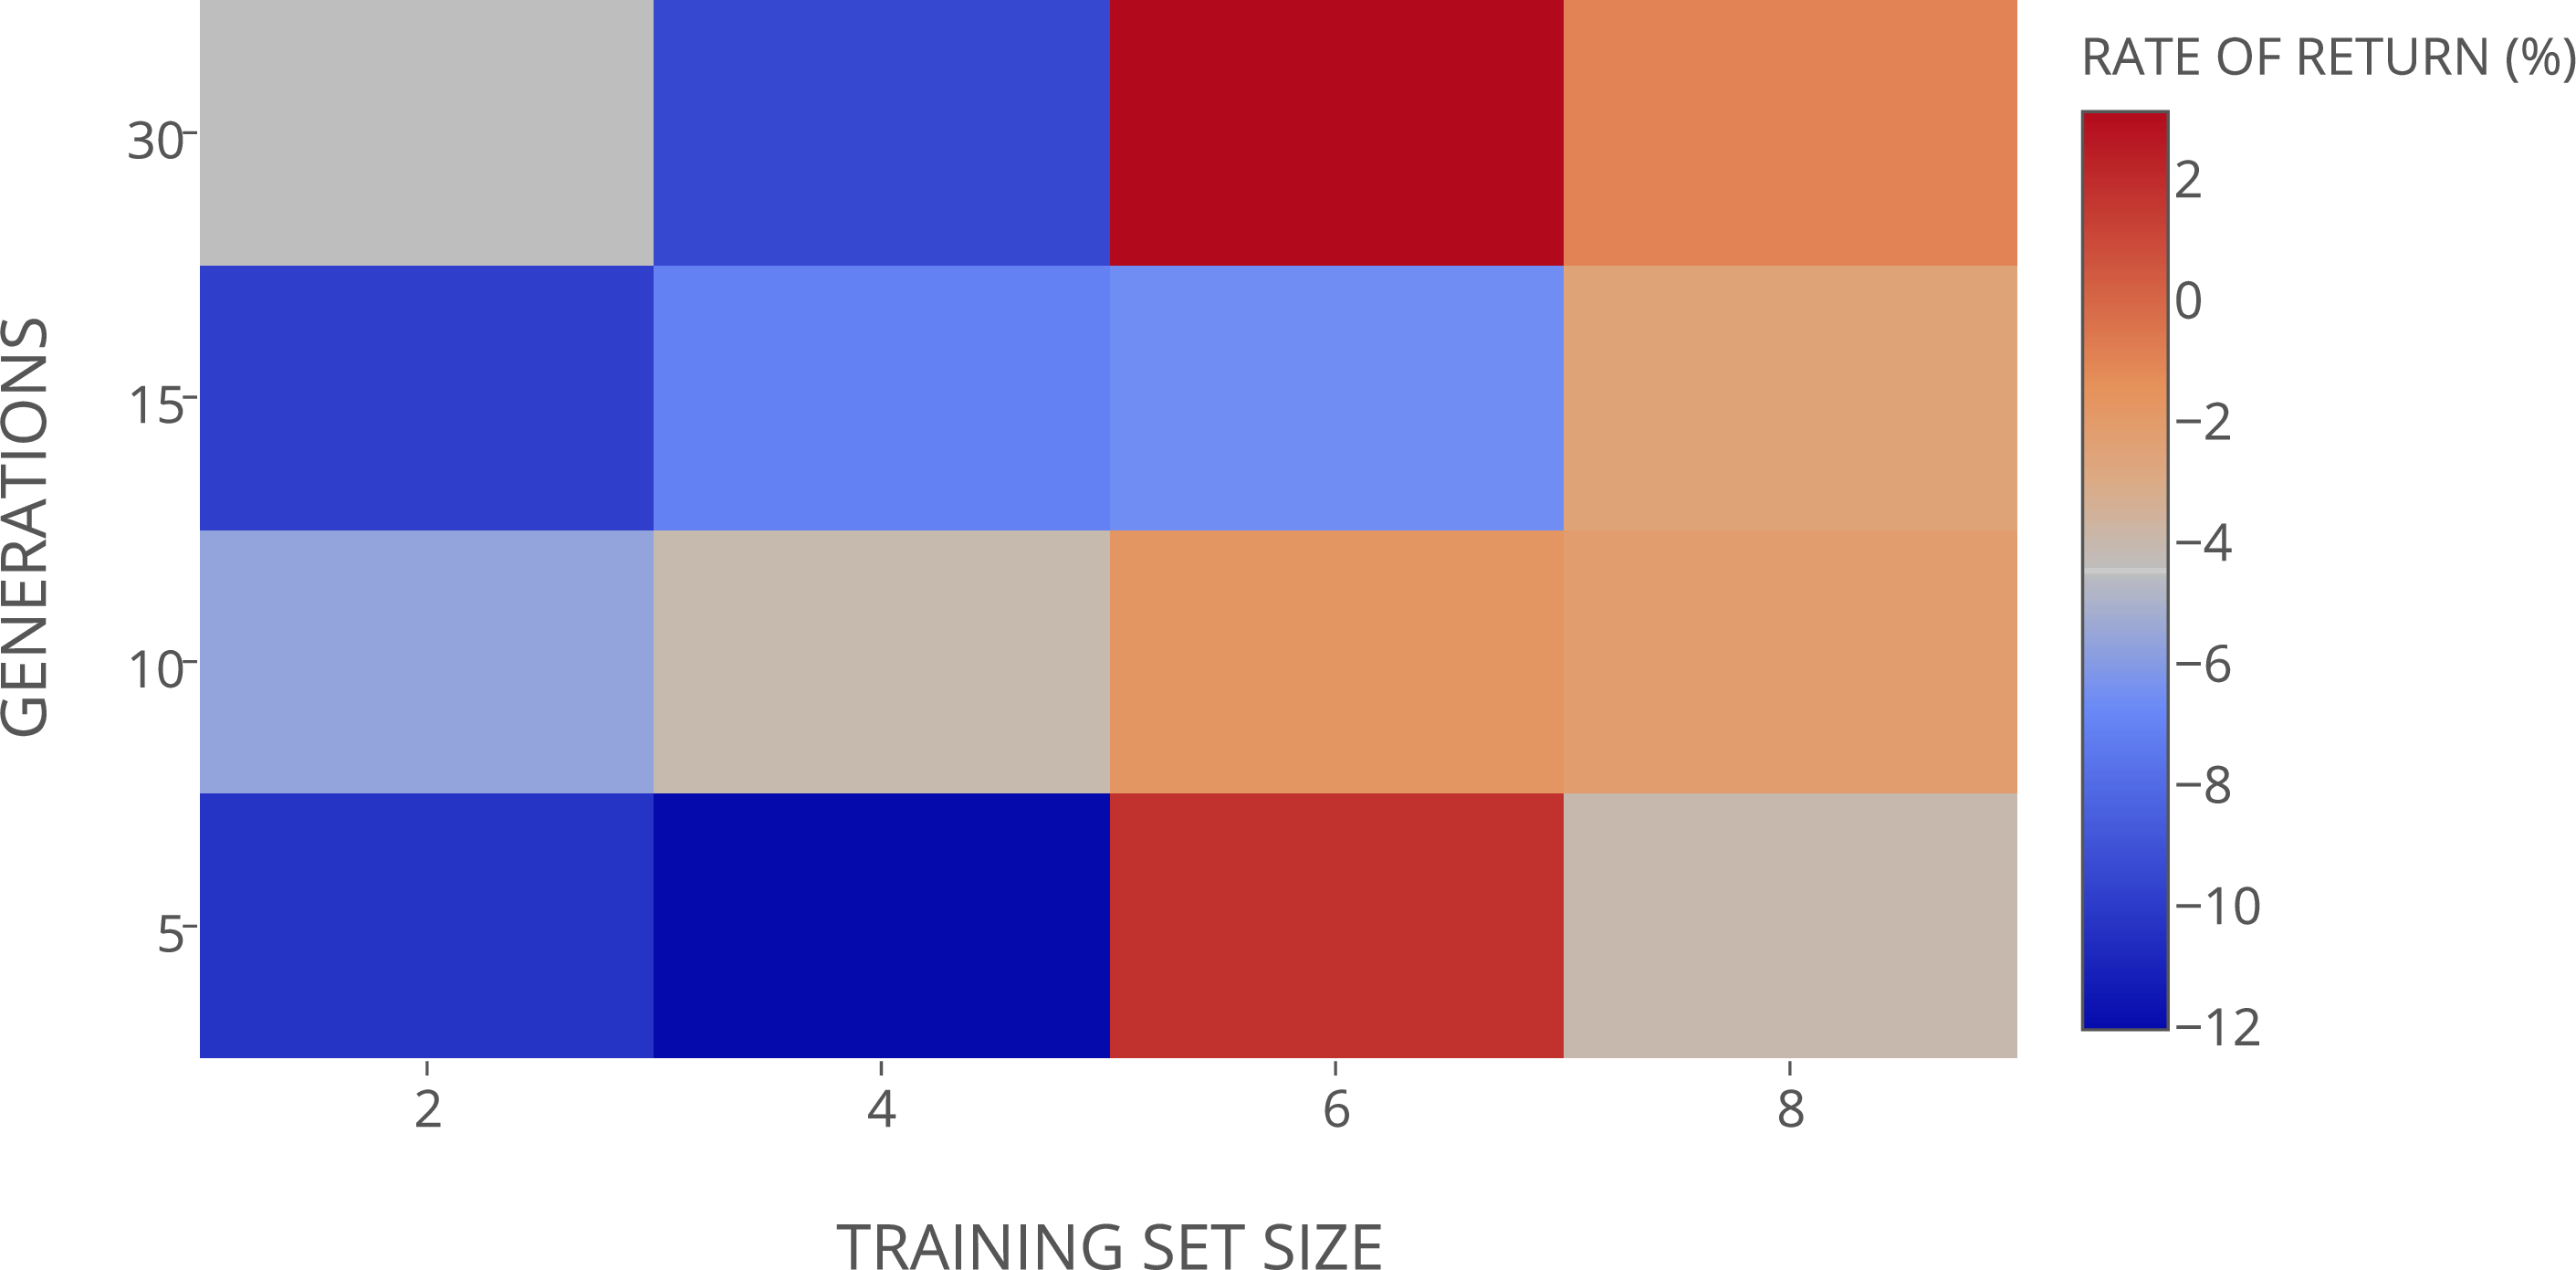
\includegraphics[width=1.00\columnwidth]{figures/rates-of-return-ibm-heatmap/rates-of-return-ibm-heatmap}
\caption{{\label{ibm-ror-heatmap}IBM Rates of Return Heatmap%
}}
\end{center}
\end{figure}

\begin{figure}[h!]
\begin{center}
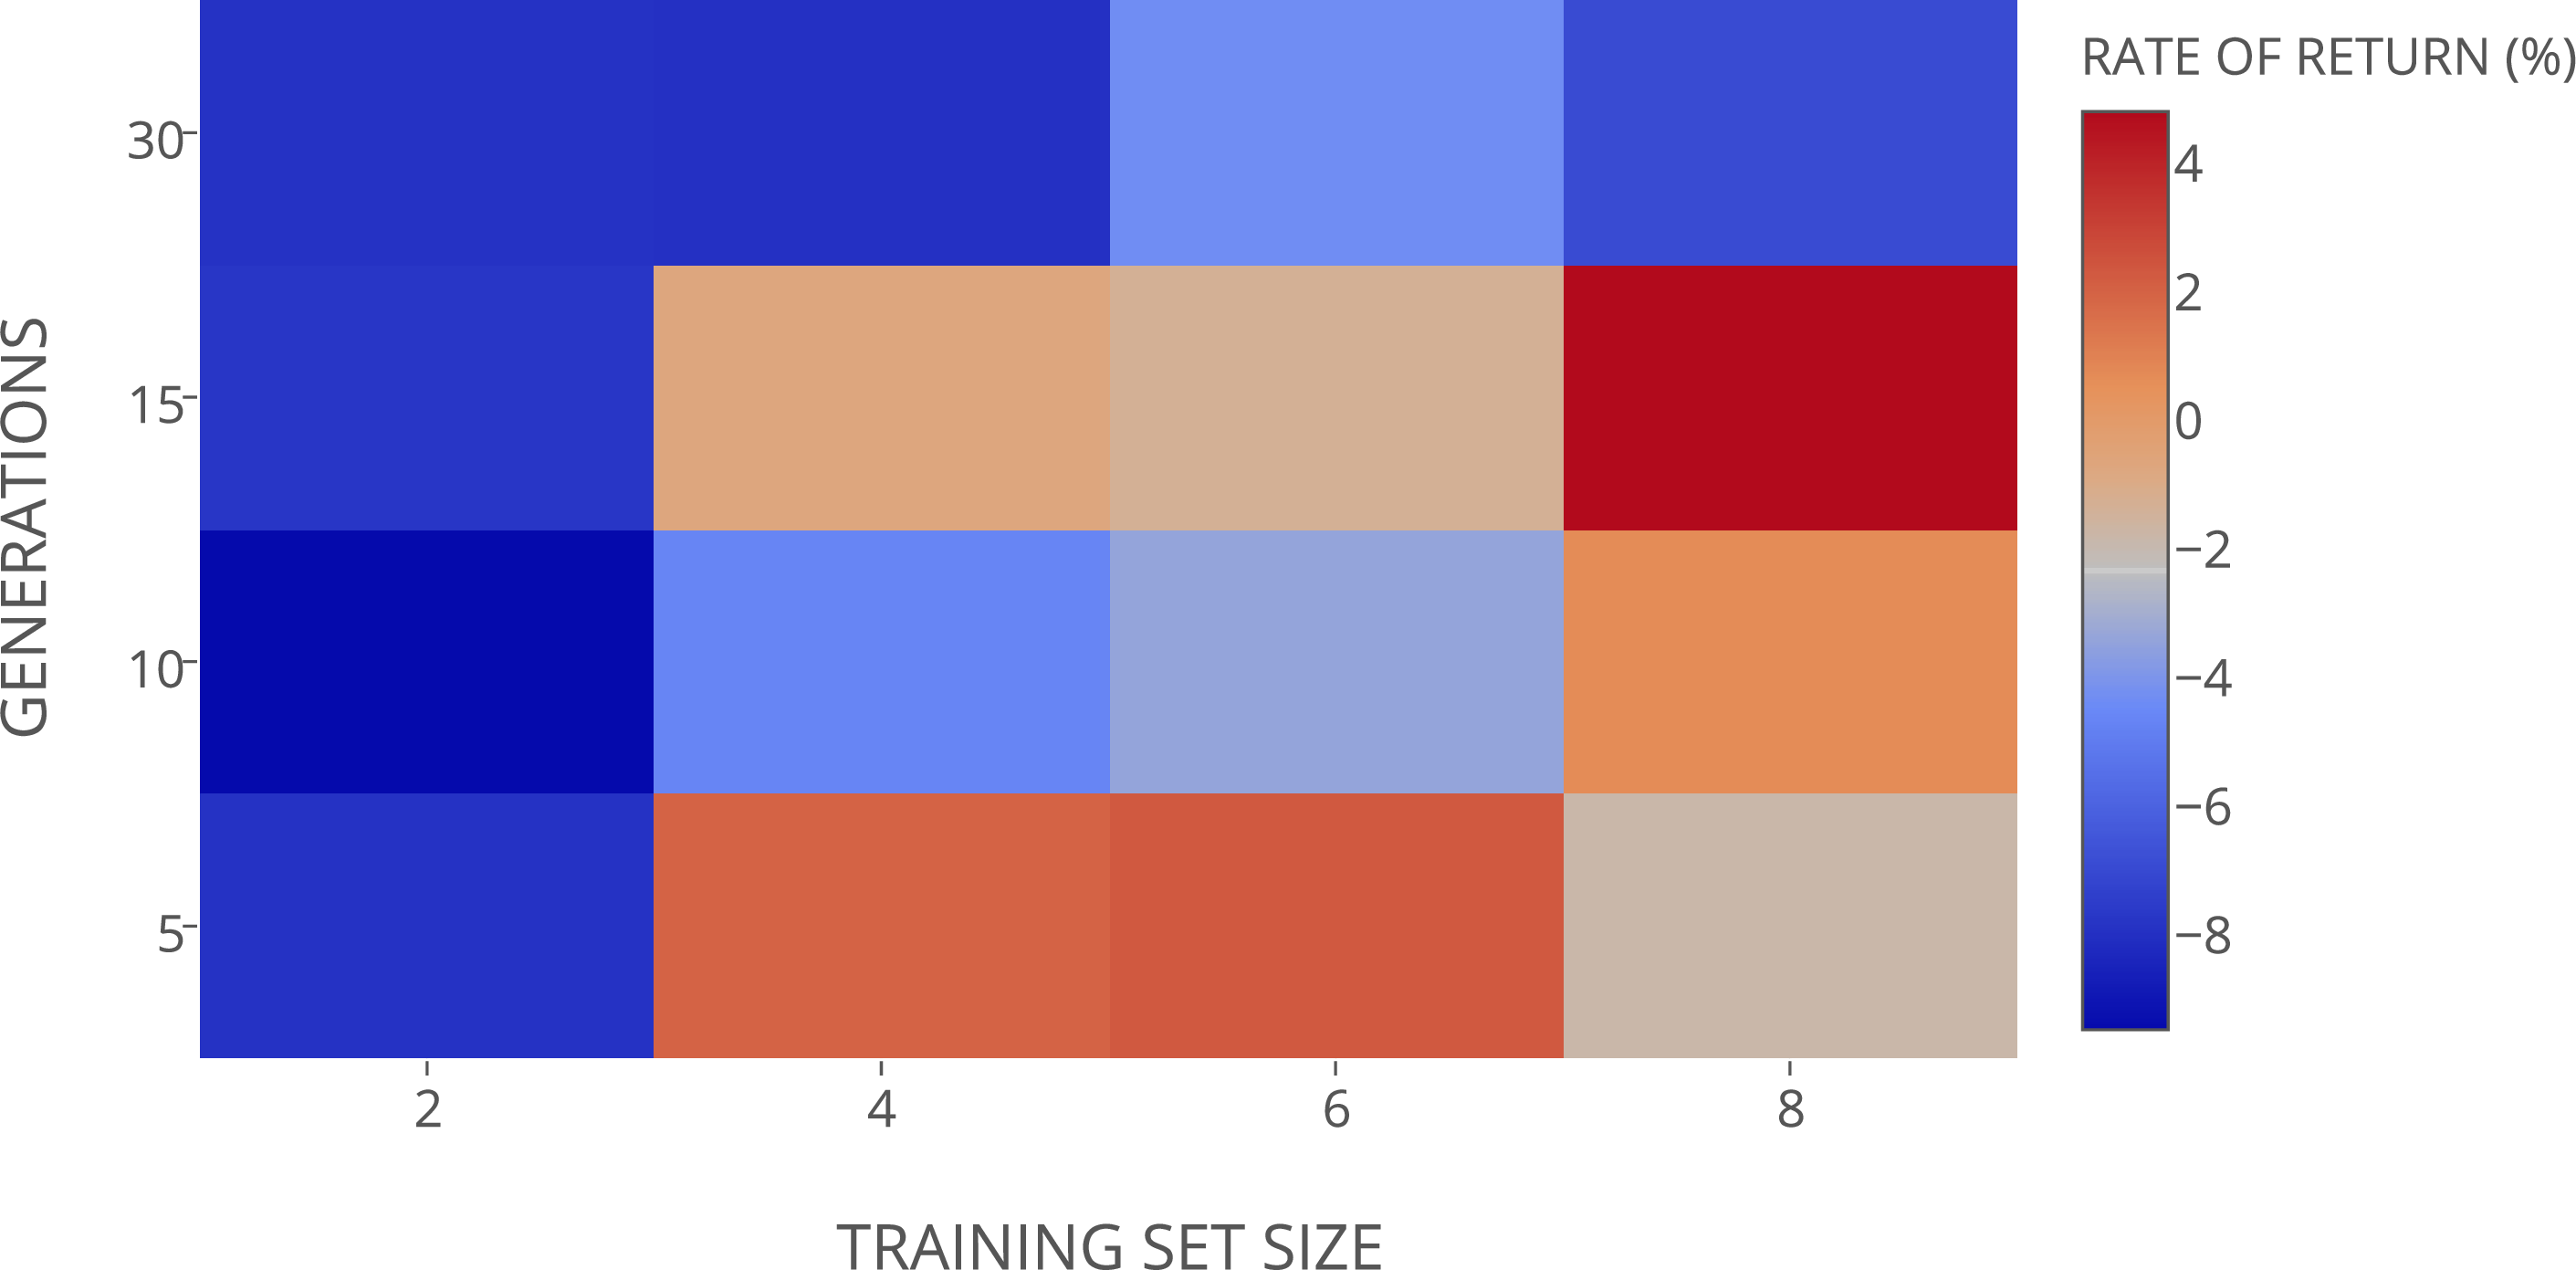
\includegraphics[width=1.00\columnwidth]{figures/rates-of-return-ko-heatmap/rates-of-return-ko-heatmap}
\caption{{\label{ko-ror-heatmap}The Coca-Cola Co. Rates of Return Heatmap%
}}
\end{center}
\end{figure}

\begin{figure}[h!]
\begin{center}
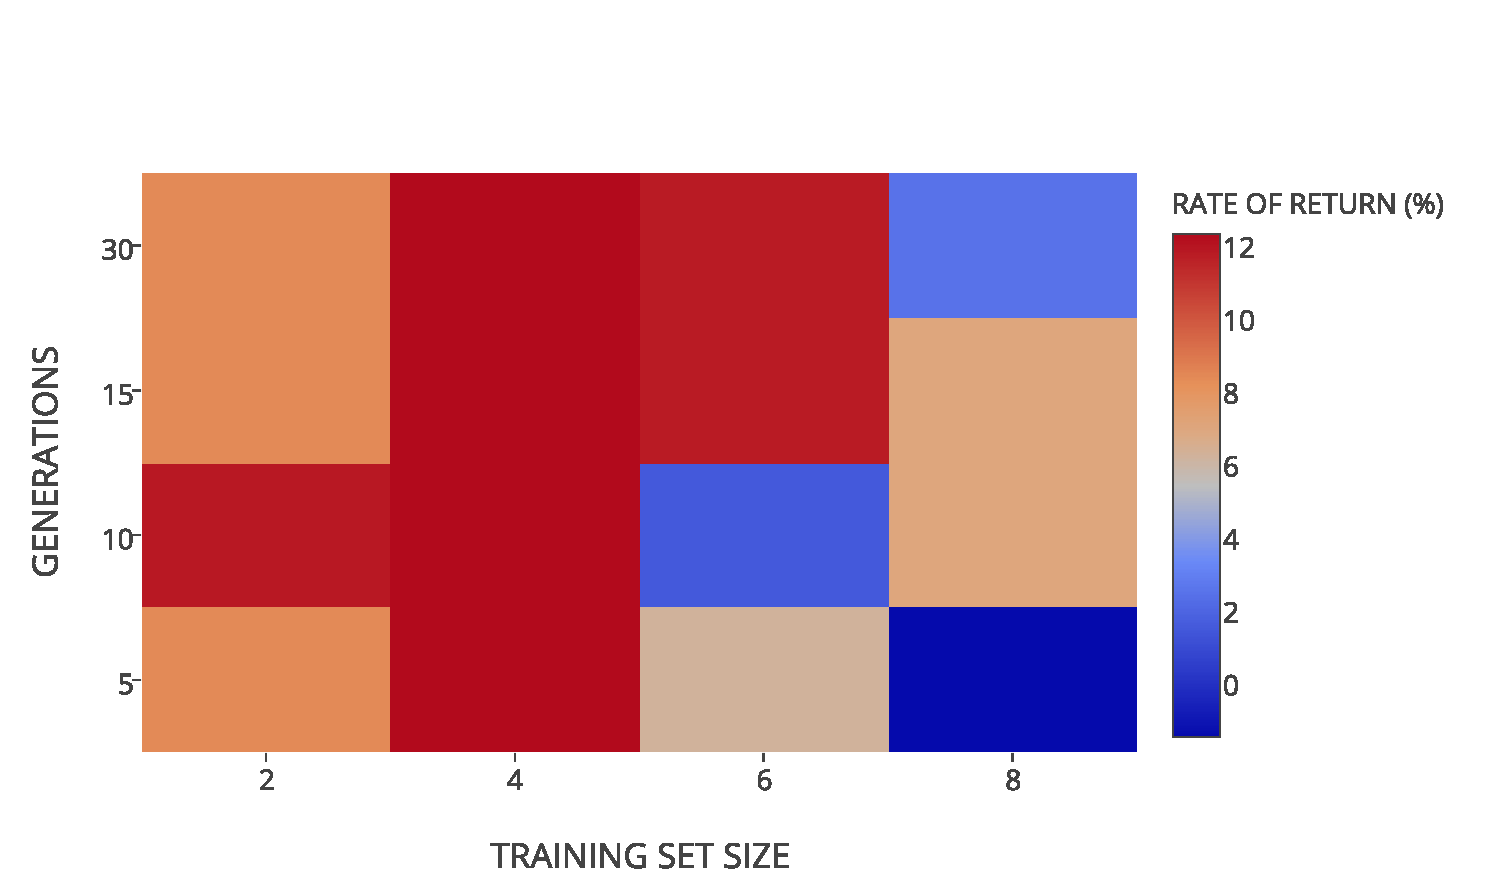
\includegraphics[width=1.00\columnwidth]{figures/rates-of-return-msft-heatmap/rates-of-return-msft-heatmap}
\caption{{\label{msft-ror-heatmap}Microsoft Rates of Return Heatmap%
}}
\end{center}
\end{figure}

\begin{figure}[h!]
\begin{center}
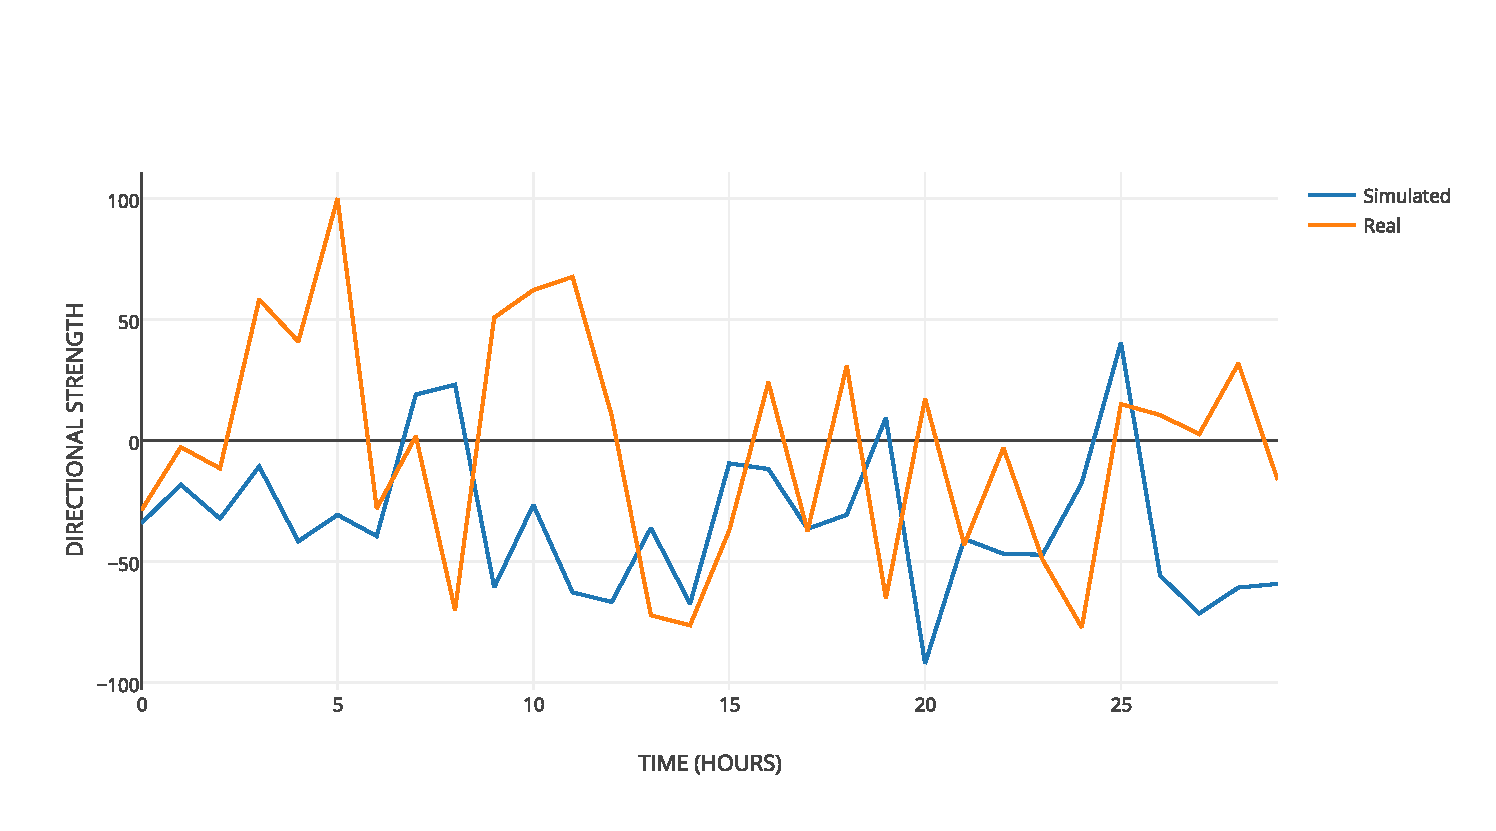
\includegraphics[width=1.00\columnwidth]{figures/ds-sim-100agents-10gen/ds-sim-100agents-10gen}
\caption{{\label{ds-prediction-10}Directional Strength Simulation - 100 Agents, 10 Generations%
}}
\end{center}
\end{figure}

\begin{figure}[h!]
\begin{center}
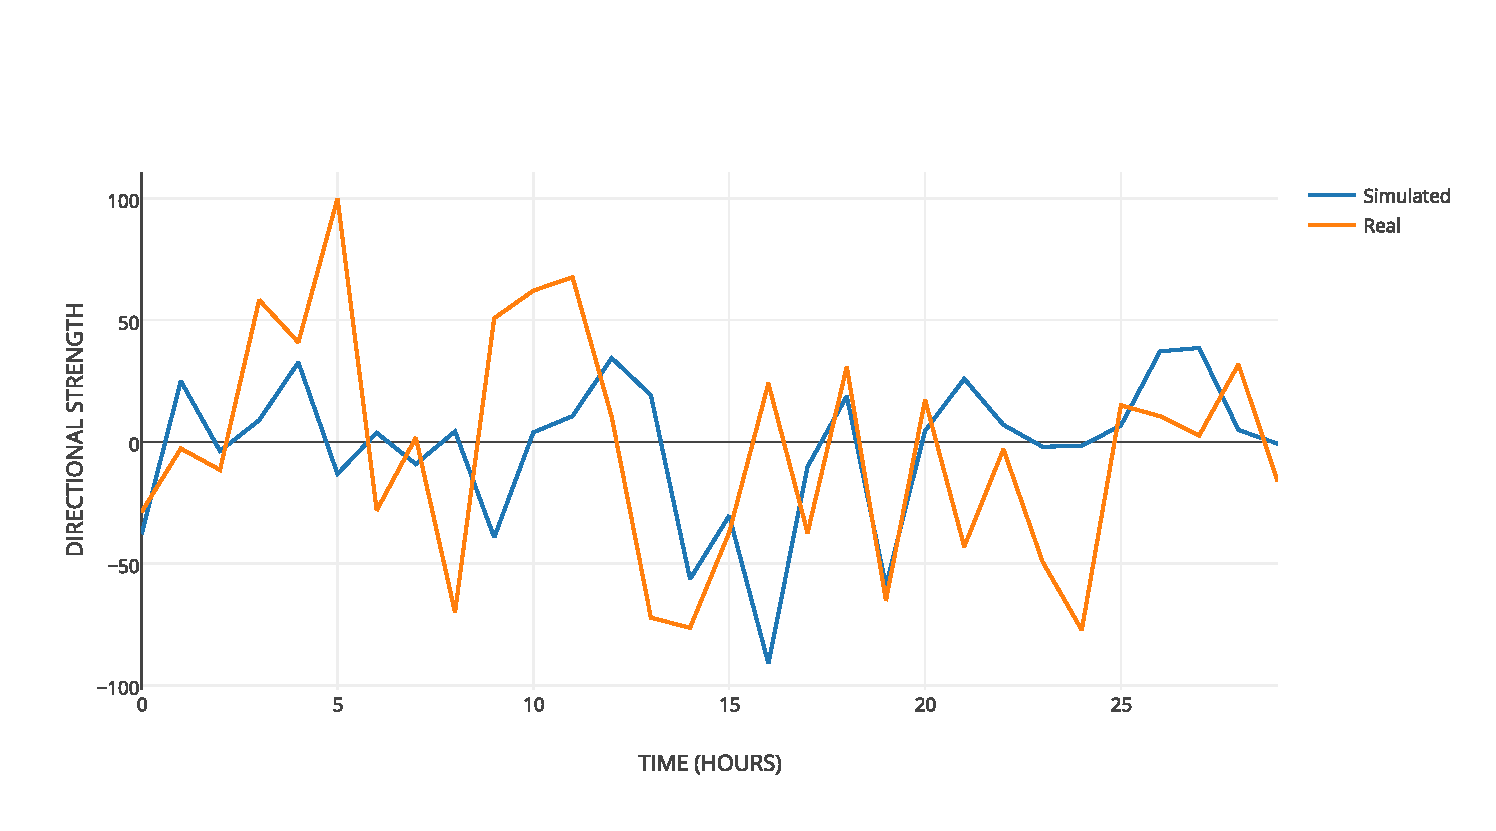
\includegraphics[width=1.00\columnwidth]{figures/ds-sim-100agents-100gen/ds-sim-100agents-100gen}
\caption{{\label{ds-prediction-100}Directional Strength Simulation - 100 Agents, 100 Generations%
}}
\end{center}
\end{figure}

\begin{figure}[h!]
\begin{center}
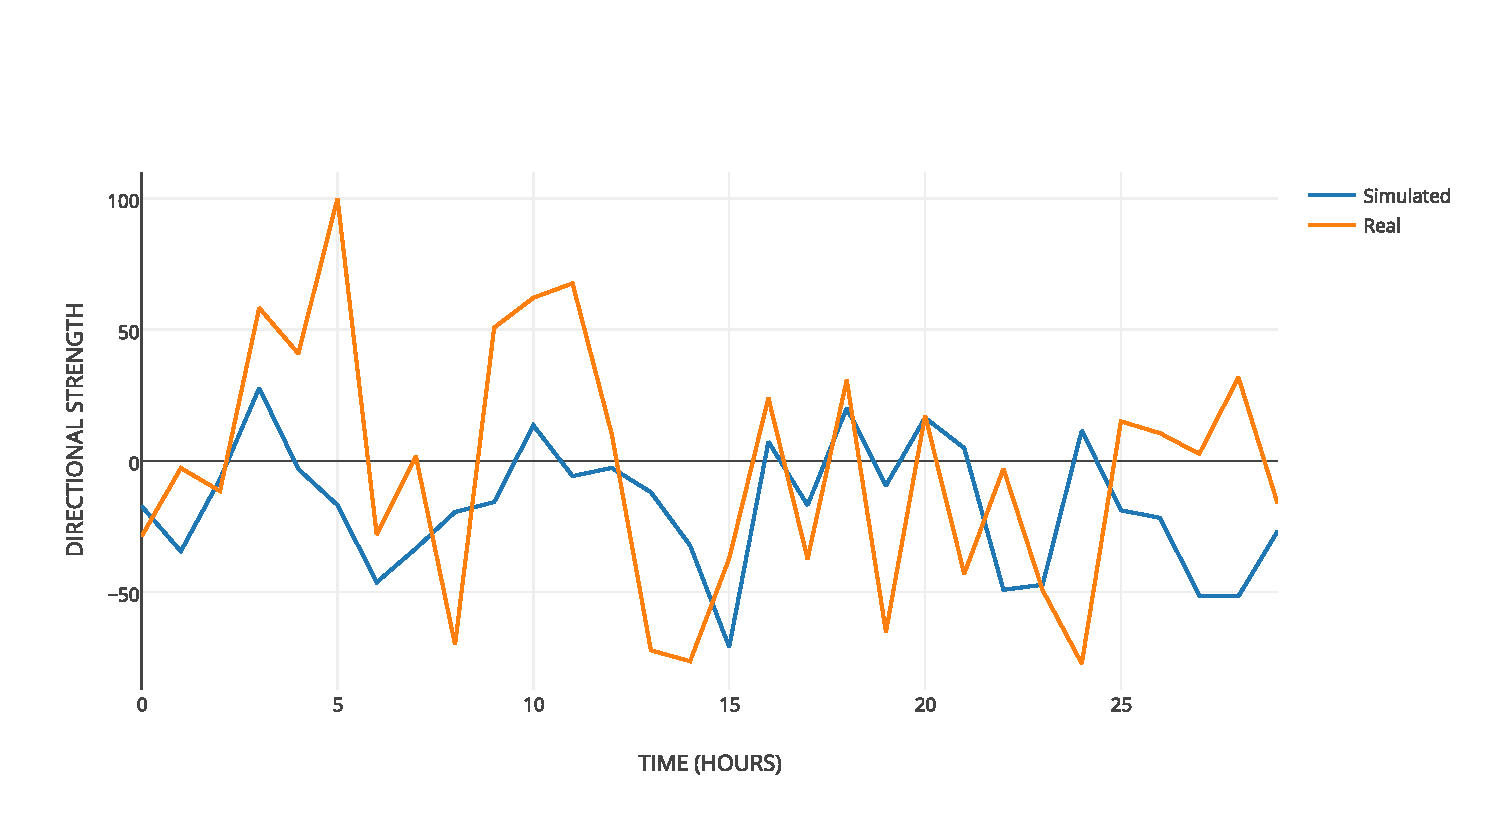
\includegraphics[width=1.00\columnwidth]{figures/ds-sim-100agents-1000gen/ds-sim-100agents-1000gen}
\caption{{\label{ds-prediction-1000}Directional Strength Simulation - 100 Agents, 1000 Generations%
}}
\end{center}
\end{figure}

\section{Conclusion and Future Work}
\label{conclusions}

The authors of this work performed exhaustive experiments in order to support the validity and efficacy of the proposed method. Nevertheless, the method should keep being validated and improved. Regarding the validation of the method, more experiments can be performed with other datasets and more comparisons with other works can be done. Regarding the improvement of the method, there are many areas of the algorithm that are known that can be improved, like applying dynamic adaptation of parameters to other parameters of the algorithm, such as the crossover, migration, and mutation chance. Also, the operators of the GP algorithm can be modified to different sets in order to obtain better performing MF, and the ranges of the literals can be adjusted (or even dynamically adapted) to improve the overall performance of the algorithm.

In conclusion, one can see that the results are very satisfactory, and that the system can effectively be used as a DSS, and as a technique to create regression models of financial time series.

\bibliographystyle{apalike}
\bibliography{bibliography/converted_to_latex.bib%
}

\end{document}

